\chapter{Hardware Validation and Demonstration}
\label{chap:HVD}

Previous chapters (Chapter \ref{chap:IS}, Chapter \ref{chap:US} and Chapter \ref{chap:HS}) focused on characterizing the performance of different CR systems jointly in terms of the interference power received by the PR and the throughput at the SR by taking the estimation of the involved channels into account. In addition, it has been motivated that the low complexity and the versatility towards unknown primary user signals requirements, facilitating hardware deployment, can be satisfied only if conventional channel estimation techniques (such as pilot-based channel estimation) are substituted with non-conventional channel estimation techniques (such as received power-based estimation, proposed in the thesis) for acquiring the channels' knowledge, particularly for the channels between the primary and the secondary systems, corresponding to different systems. However, the aforementioned analysis in the previous chapters has been limited to the theoretical expressions. 


With regard to the analytical expressions that are necessary for the performance analysis, it is essential as-well-as challenging to depict the hardware realizability of CR systems. Motivated by this fact, this chapter, which is based on \citeK{Kaushik15_ICC, Kaushik16_CC}, reconciles the theory established in the previous chapters and the hardware feasibility of the CSC. As a result, to a great extent, this chapter complements the performance analysis by deploying the CR techniques on a hardware. By doing this, the applicability of the assumptions considered while deriving the analytical expressions can be examined. Moreover, these investigations facilitate the evolution of the proposed analytical framework. Without any specific argumentation, an US is considered for the deployment.    
%%\begin{abstract}        % give a summary of your paper
%Cognitive radio is one of the potential contenders that address the problem of spectrum scarcity by making efficient use of the currently allocated spectrum below \SI{6}{GHz}. A secondary access to the licensed spectrum is only possible, if the cognitive radio systems restrict the interference to the primary systems. However, the performance analysis of such a cognitive radio system is a challenging task. Currently, performance evaluation of underlay systems is limited to theoretical analysis. Most of the existing theoretical investigations make certain assumptions in order to sustain analytical tractability, which could be unrealistic from the deployment perspective. Motivated by this fact, in this work, we validate the performance of an underlay system by means of laboratory measurements, and consequently propose a hardware demonstrator of such a system. Moreover, we present a graphical user interface to provide insights to the working of the proposed demonstrator and highlight the main issues faced during this experimental study.
%\blfootnote{This work was partially supported by the National Research Fund, Luxembourg under the CORE projects "SeMIGod" and "SATSENT".} 

% please supply keywords within your abstract
%\keywords {Cognitive Relay, underlay system, power control, dynamic access, empirical validation, demonstrator}
%\end{abstract}



%\section{Related Work}

%The amount of data transmitted over wireless channels is constantly increasing. However, the available spectrum is scarce and expensive, with more and more operators competing for their share of it. Therefore, ways have to be found to use the available spectrum more efficiently. Cognitive radio networks do so by enabling dynamic spectrum access to multiple systems. Secondary access to the licensed spectrum has been extensively investigated in the literature and is mainly categorized in terms of three cognitive radio paradigms \cite{Goldsmith09}: 
%\begin{enumerate}
%	\item An interweave system exploits time gaps in the spectrum of primary users for data transmission. 
%	\item An overlay system involves higher network layers to employ advanced coding algorithms to transmit data simultaneously with other systems. 
%	\item In an underlay system, spectrum access is enabled only if the interference power received at primary users is below a certain amount. This can be achieved, for instance, by employing a power control mechanism at the secondary transmitter. 
%\end{enumerate}

%The existing investigations in \cite{Ghasemi07, Xin09, Musa09} depicted the performance limits in terms of throughput achieved at the secondary receiver for the underlay system. However, the performance evaluation has been limited to theoretical analysis, which tends to make certain assumptions (for instance, perfect knowledge of channel), that are not applicable in hardware implementations \cite{Sharma15}. Recently, hardware implementations in context to cognitive radio systems have started to receive significant attention \cite{Ngu13, Anas12, Combes15}, however these deployments are mainly concerned with the interweave system. In this regard, we provide insights for the deployment of underlay systems, in this paper. More specifically, we extend the mathematical framework derived in \cite{Kaushik15} to validate the performance of underlay systems by means of experimental analysis. To complement the analysis presented in \cite{Kaushik15}, 

In this regard, this chapter provides the following contributions:
\begin{itemize}
	\item \index{Hardware validation}Empirical validation: The performance of the USs in accordance to the received power-based estimation employed for the channel between the PR and the ST is validated by means of a hardware deployment. The variations (induced due to incorporation of channel estimation) in the system parameters are validated by comparing their probability density functions, obtained from the measurements, to those computed analytically. Moreover, the joint performance of the underlay system is validated in terms of an \index{Tradeoffs!estimation-throughput tradeoff}estimation-throughput tradeoff, proposed in Chapter \ref{chap:US}. %A suitable hardware environment is establish to perform measurements and evaluate their results by comparing them with the theoretical expressions.
	\item Demonstrator\index{Demonstrator}: Upon validating the theoretical expressions, a hardware demonstrator following the guidelines of an US is deployed. In this context, the applicability of the proposed framework in realistic scenarios is justified. Further, a graphical user interference\index{Graphical user interface} is designed to procure insights on the operation of the demonstrator.	
\end{itemize}

%This paper is organized as follows: Section \ref{sysmod} introduces the system model. Section \ref{val} describes the experimental setup and the validation of the mathematical model. Section \ref{demo} portrays the implementation of the underlay system's hardware demonstrator. Finally, Section \ref{con} concludes the paper.


\section{System Model}
\label{sysmod}

\subsection{Model Simplifications}
\label{ssec:simp1}
In contrast to the framework presented in Chapter \ref{chap:US}, the following simplifications and modifications are considered for the hardware implementation.
\begin{itemize}
\item The channel estimation (received power-based) is only deployed for the link between the PR and the ST, which is associated with the interference received at the PR. In order to simplify the deployment, the interference from the PTs at the SR is neglected. Although the knowledge of the interference from the PTs is essential for characterizing the secondary throughput, the knowledge of the interference at the PR is critical for the imposition of the PU constraints. In addition, perfect knowledge of the access channel between the ST and the SR that employs the pilot-based channel estimation is considered\footnote{In contrast to the received power-based estimation, the employment of pilot-based channel estimation has an negligible effect on the performance degradation in terms of the time allocated within the frame structure and the amount of variations induced. In this context, perfect channel estimation for access channel presents a reasonable assumption.}.  
\item The measurements taken to perform the validation, and the demonstration for the proposed deployment scenario consider the deterministic behaviour of the interference channel.  
\item As an alternative to the outage constraint, proposed in Chapter \ref{chap:US} for regulating the uncertain interference at the PR, a \index{Interference constraint!confidence probability constraint}confidence probability constraint is employed for capturing the variations due to channel estimation around the interference temperature. %Moreover, previous analysis considers the realization of the power control over multiple frame. Here, the power control subject  
\item Lastly, in contrast to the \index{OFDM}OFDM signal considered in Chapter \ref{chap:US}, in this chapter all transmit signals (which include pilot and data signals) at the primary and the secondary systems are modeled as a constant power signal. 
\end{itemize}

In accordance to these simplifications, the system model for the US depicted in Chapter \ref{chap:US} is slightly modified. 

\subsection{Underlay Scenario and Medium Access}
%\todo{Update \figurename~\ref{fig_HVD:scenario}}
\label{scenario}

\begin{figure}
	%\vspace{-10 pt}
	\centering
	\subfloat[]{
	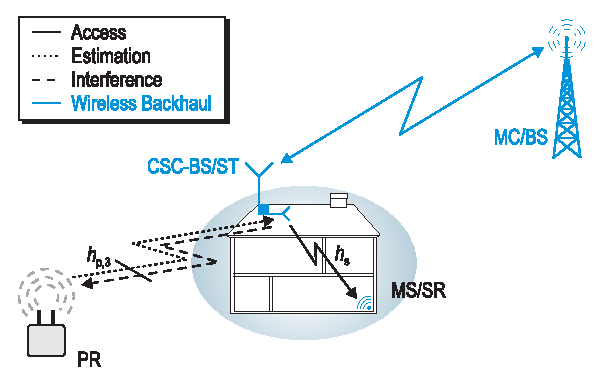
\includegraphics[width=0.55\textwidth]{figures/CR_Scenario_Underlay_gruen}%
	}
	\subfloat[]{
	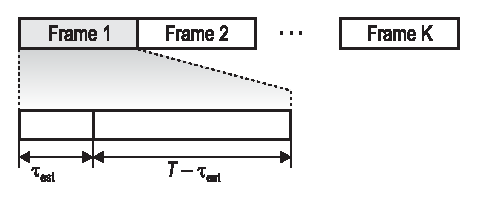
\includegraphics[width=0.45\textwidth]{figures/Frame_Structure_grau_U}%
	}
	\caption{ With regard to Chapter \ref{chap:US}, a simplified illustration of (a) the CSC scenario demonstrating an underlay paradigm. (b) Frame structure from the perspective of the ST that presents a time duration ($\test$) allocated for the estimation of the interference channel.} 
	\label{fig_HVD:scenario}
	%\vspace{-10 pt}
\end{figure}



%\figurename~\ref{fig_HVD:scenario} depicts a CSC deployment consisting of a CSC-BS, a MS, a PR and a MC-BS. Analog to the previous scenarios, the CSC-BS and the MS represent a ST and a SR. 

In accordance with Chapter \ref{chap:US}, the channels between the PR and the ST and between the ST and SR are designated as the interference and the access channels with channel gains $\hpth$ and $\gs$, respectively. A power control mechanism is employed at the ST to ensure that interference received at the PR is below a certain level. In order to exercise power control mechanism, it is necessary to acquire the knowledge of the channel between the ST and the PR. As proposed in Chapter \ref{chap:US}, the ST can retrieve this information by listening to a pilot or beacon signal transmitted by the PR. %For the received pilot signal ($y_\textrm{rcvd}$) and its power, we use the model and notations from \cite{Kaushik15}.


A slotted medium access is implemented at the ST with a frame duration of $T$. The knowledge of the interference channel is acquired by employing \index{Channel reciprocity}channel reciprocity over the link PR-ST. %Besides, $T$ is selected such that the channel can be assumed to remain constant for the frame duration. %Based on this premise, $g_\textrm{p}$ and $g_\textrm{s}$ are constant within one frame and included in $\alpha_\textrm{p}$ and $\alpha_\textrm{s}$ for further analysis.
In order to incorporate channel estimation in context to the power control mechanism, the frame interval is divided in two phases, namely estimation and data transmission, refer to \figurename~\ref{fig_HVD:scenario}. During the estimation phase $\test$ (also referred as estimation time), the ST measures the received power of the signal (a pilot signal with known transmit power, refer to Section \ref{ssec_US:as} in Chapter \ref{chap:US} for a detailed discussion) transmitted by the PR. Based on this received power, the ST implicitly acquires the knowledge of $\phpth$, using which it controls its transmit power for the secondary link while satisfying a constraint on the interference received by the PR. During the data transmission phase $T-\test$, the ST transmits data with the controlled power to the SR.

\subsection{Signal Model}
The discrete and complex signal received at the ST is given by
%ived signal at the ST, transmitted by the PR cf. \figurename~\ref{fig_HVD:scenario}, is sampled with a sampling frequency of $\fsam$ and is given by
\begin{equation}
\yrcvd[n] = \hpth \cdot \xtranpr[n] + \wst[n],
\label{eq_HVD:sys_mod_st}
\end{equation}
where $\xtranpr[n]$ corresponds to a discrete and complex \index{Constant power signal} constant power signal transmitted by the PR, $\phpth$ represents the power gain for the channel PR-ST and $\wst[n]$ is circularly symmetric AWGN at the ST.
 $\ptranpr$  corresponds to the transmit power at the PR and $\wst[n]$ is a Gaussian random variable with $\e{}{\wst[n]} = 0$ and $\e{}{|\wst[n]|^2} = \nps$. 

By listening to the transmissions from the PR, the estimated received power at the ST, computed using $\test \fsam$ samples, is given as
\begin{align}
\eprcvdstpr = \s{\test \fsam}{ |\hpth \cdot \xtranpr[n] + \wst[n]|^2},
\label{eq_HVD:prcvd} 
\end{align}
where $\fsam$ denotes the sampling frequency. 

After implementing the power control at the ST, during the data transmission, the received signal at the PR is given by
\begin{equation}
\yp[n] = \hpth \cdot \xscont[n] + \wpr[n],
\label{eq_HVD:sys_mod_pr}
\end{equation}
and, on the other side, the received signal at the SR follows
\begin{equation}
\ys[n] = \gs \cdot \xscont[n] + \wsr[n],
\label{eq_HVD:sys_mod_sr}
\end{equation}
where $\xscont[n]$ presents the signal with controlled power ($\preg$) at the ST. 

During the data transmission phase, the controlled power at the ST is determined as 
\begin{align}
\epreg = \s{(T - \test) \fsam}{|\xscont[n]|^2} 
\label{eq_HVD:preg} 
\end{align}
Further, $\phpth$ and $\pgs$ represent the power gains for the channels ST-PR and ST-SR, respectively, cf. \figurename~\ref{fig_HVD:scenario}. 

During the data transmission phase, the received powers at the PR and the SR are evaluated as 
\begin{align}
\eprcvdpr &= \s{(T - \test) \fsam}{|\yp[n]^2|}  \intertext{ and} \eprcvdsr 
&= \phs \epreg, %\s{(T - \test) \fsam}{|\ys[n]^2|}, 
\end{align}
respectively. Likewise (\ref{eq_HVD:sys_mod_st}), $\wpr[n]$ and $\wsr[n]$ represent circularly symmetric \index{AWGN}AWGN at the PR and the ST with zero mean and variance $\e{}{|\wpr[n]|^2} = \e{}{|\wsr[n]|^2} = \npp$, respectively. %Consider that $\ptran$, $\preg$ and $\pp$ correspond to power for a given frame. 
%For (\ref{eq_HVD:sys_mod_sr}), we assume that the interference at SR from the PR via beacon or pilot channel is $< \nps$, which is a valid assumption considering the indoor scenario depicted in \figurename~\ref{fig_HVD:scenario}. 
%For (\ref{eq_HVD:sys_mod_sr}), we consider a perfect allignment of the ST to the beacon or pilot channe
%\subsubsection{Channel}

After utilizing $\test$ for channel estimation, the throughput at the SR over the access channel\footnote{Please note, it is assumed that the access channel is perfectly known at the ST and SR procures no interference from the PT.} is given by
\index{Secondary throughput}
\begin{equation}
\ers = \frac{T - \test}{T} \log_2 \left(1 + \frac{\pgs \epreg }{\nps} \right). 
\label{eq_HVD:sthr}
\end{equation}


%All transmitted signals are subjected to distance dependent path loss and small scale fading gains depicted as $\hpth, \gs$. In the analysis, the coherence time of the channels $\approx T$ is considered. But, there will be scenarios where the coherence time exceeds $T$, in such cases the expressions derived in this chapter depicts a lower performance bound.


\section{Theoretical Analysis}
\label{model}
In order establish a close relationship between the analytical framework and the hardware implementation, the sequence of events depicted by the underlay scenario in \figurename~\ref{fig_HVD:scenario} are summarized as follows:

\begin{enumerate}
	%\item The PR sends a pilot signal with power $\ptranpr$ to the ST.
	\item The ST estimates the power received $\eprcvdstpr$ (i.e., employs \index{Channel estimation!received power based}received power-based estimation) by listening to the pilot signal transmitted by the PR over the interference channel. In the context of the hardware implementation, an unmodulated sinusoidal signal is sent as a pilot or beacon signal. 

Please note that a sinusoidal signal is mathematically equivalent to the constant power signal sent by the PR, resembling a continuous phase modulated signal (for instance, a minimum shift keying signal) or a discrete phase modulated signal (for instance, a \index{Phase shift keying}phase shift keying signal), which represents a perfectly downsampled signal. For the latter case, perfect implies an appropriate selection of the sampling point so that no inter symbol interference is procured by the system (in other words, \index{Nyquist criterion}Nyquist criterion is satisfied). In correspondence to the signal model that assumes i.i.d. samples, such a requirement is essential for the evaluation of the received power (energy detection or received power-based estimation), which is necessary for validating the theoretical expressions, derived in the thesis.
	\item With the knowledge of $\ptranpr$ and the estimate $\eprcvdstpr$, the ST indirectly acquires the knowledge of $\phpth$. 
	Upon acquiring this knowledge, a power control is employed at the ST. Using $\eprcvdstpr$, $\epreg$ is determined as 
\begin{align}
\epreg = \frac{\ite K}{\eprcvdstpr}, \label{eq_HVD:preg} 
\end{align}
where $K$ represents a \index{Scaling factor}scaling factor. The scaling factor is required at the ST to hold $\e{}{\eprcvdpr}$ at $\ite$. It is defined as
\begin{align}
K = \frac{1}{ \e{\eprcvdstpr}{\frac{\phpth}{\eprcvdstpr}}}, \label{eq_HVD:sca} 
\end{align}
where $\e{\eprcvdstpr}{\cdot}$ represents the expectation over $\eprcvdstpr$.
	%It is scaled such that, in case of perfect channel reciprocity and the absence of noise on the primary link, the interference power arriving at the PR ($\prcvdpr$) has the value of the interference temperature ($\ite$). %In control theory terms, $\ite$ is the setpoint for $\prcvdpr$.
	\item The ST transmits data to the SR at $\epreg$. 
	%\item The SR receives the data signal with power $\preg$ It provides this value back over a feedback channel to the ST, where it is used to estimate the expected secondary throughput $\e{\rs}{\rs}$ over the access channel.
	The estimated power (represented as $\eprcvdstpr$) over the interference channel induces variations in the controlled power (represented as $\epreg$). With regard to the relation between the controlled power at the ST and the received power at the PR, represented as 
\begin{align}
\prcvdpr  = \phpth \preg,
\label{eq_HVD:eprcvdpr}
\end{align}
the variations in $\epreg$ translate to the variations in $\prcvdpr$ (represented as $\eprcvdpr$) around $\ite$, resulting in uncertain interference at the PR. Unless captured, these variations may severely degrade the performance of the US. Besides this, due to the relationship between the controlled power and the secondary throughput, defined in (\ref{eq_HVD:sthr}), the variations are further translated to the secondary throughput. 
\item These variations in the system parameters ($\eprcvdstpr$, $\epreg$, $\eprcvdpr$ and $\ers$) are characterized in terms of their pdfs. In particular, the pdf of $\eprcvdpr$ is utilized to employ an interference constraint (also referred as confidence probability constraint) in terms of confidence probability $\pco$ at the ST so that the uncertain interference at the PR can be regulated effectively. In addition, by utilizing the pdf of $\ers$, the performance of the access channel is determined in terms of the expected secondary throughput. \item Finally, subject to the confidence probability constraint, the performance of the US is jointly characterized in terms of a tradeoff between the estimation time and the secondary throughput. 
\end{enumerate}

\subsection{Characterization of the System Parameters}
In order to capture the variations induced due to channel estimation, the pdfs of the aforementioned system parameters ($\eprcvdstpr$, $\epreg$, $\eprcvdpr$, $\ers$) are characterized, subsequently. 

In accordance to the employed signal model, $\prcvdstpr$ is modeled as a non-central chi-squared distribution $\ncchi2$, whose pdf is characterized as \cite{Char99}
\begin{align}
	\label{eq_HVD:dprcvdstpr}
	\dprcvdstpr (x) =& 
	\frac{\test \fsam}{2\npp} \left(\frac{\test \fsam x}{\lambda}\right)^\frac{\test \fsam-2}{4} \exp\left(-\frac{\test \fsam x+\lambda}{2\npp}\right)  \times \\ 
	\quad & I_{ \frac{\test \fsam}{2}-1 }\left(\frac{\sqrt{\test \fsam x \lambda}}{\npp}\right) \nonumber  ,
\end{align}
where $\test \fsam$ is the degree of freedom and also the number of complex samples used for the estimation. $\npp$ is the noise variance of the in-phase and the quadrature-phase components of the received pilot signal ($\yrcvd[n]$, refer to \ref{eq_HVD:sys_mod_st}), and $I_{\frac{\test \fsam}{2}-1}(\cdot)$ is the modified \index{Bessel function}Bessel function of the first kind of order $\frac{\test \fsam}{2}-1$ \cite{Jef00}. Furthermore, the non-centrality parameter is defined as
\begin{equation}
	\label{lambda}
	\lambda = \sum_{n=1}^{\test \fsam} \mathbb{E}[|\yrcvd[n]|^2] = \test \fsam \times A^2.
\end{equation}
The evaluation of $\lambda$ in (\ref{lambda}) can be explained as follows: a sinusoidal signal that represents a pilot signal consists of a constant amplitude, which is downconverted by an I/Q demodulator at the ST. In this regard, the complex samples $\yrcvd[n]$ have a constant envelope of value $A$. 

Corresponding to (\ref{eq_HVD:preg}), $\epreg$ follows an inverse non-central chi-squared distribution. The pdf for $\epreg$  is given by
\begin{align}
\dpreg(x) =& \frac{\test \fsam K \ite}{2\npp x^2} e^{- \frac{\tau \fsam}{2 \npp}\left( \frac{K  \ite}{x} + \phpth \ptran \right)} \left( \frac{K \ite}{x \phpth \ptran}   \right)^{\frac{\test \fsam}{4} - \frac{1}{2}} \label{eq_HVD:dpreg} \times \\
\quad & I_{\frac{\test \fsam}{2}  - 1}\left( \frac{\test \fsam}{\npp} \sqrt{\frac{ K \ite \phpth \ptran}{x}}  \right). \nonumber
%\fpreg(x) = \q{\frac{N}{2} - 1}{\sqrt{\frac{N \ptran \ap}{\npp}},\sqrt{\frac{N \cdot x}{\npp}} }, 
\end{align}
%where $\q{\frac{N}{2} - 1}{\cdot, \cdot}$ is the Marcum-Q function \cite{grad}.
%where $I_{\frac{N}{2}  - 1}(\cdot)$ represents the Bessel function of order $\frac{N}{2} - 1$ \cite{grad}.

Following the relation in (\ref{eq_HVD:eprcvdpr}) and substituting $\dpreg(x)$, defined in (\ref{eq_HVD:dpreg}), the pdf of $\eprcvdpr$ is determined as 
\begin{align}
\dprcvdpr(x) =& \frac{\phpth \test \fsam K \ite}{2\npp x^2} e^{- \frac{\test \fsam \phpth}{2 \npp}\left( \frac{K  \ite}{x} + \ptran \right)} \left( \frac{K \ite}{x \ptran}   \right)^{\frac{\test \fsam}{4} - \frac{1}{2}} \times \label{eq_HVD:dpp} \\
\quad & I_{\frac{\test \fsam}{2}  - 1}\left( \frac{\test \fsam \phpth}{\npp} \sqrt{\frac{ K \ite \ptran}{x}}  \right). \nonumber
\end{align}

%The definition of $P_\textrm{c}$ can be retrieved from \cite{Kaushik15}. 
Consequently, the cdf of $\eprcvdpr$ is given by %\footnote{In \cite{Kaushik15}, we discovered a small typing error in the cdf of $P_\textrm{p}$, in this paper, we present the exact version of it.}
\begin{equation}
	\label{eq_HVD:cdf}
	\fprcvdpr(x) = Q_{\frac{\test \fsam}{2}}\left(\sqrt{\frac{\test \fsam \ptran \phpth}{\npp}},\sqrt{\frac{\test \fsam \phpth \ite K}{\npp x}}\right) \;  ,
\end{equation}
where $Q_{\frac{\test \fsam}{2}}(\cdot)$ is the \index{Marcum Q-function}Marcum Q-function \cite{Jef00}.

%The system variables $P_\textrm{cont}$, $P_\textrm{p}$, and $R_\textrm{s}$ are derived from $P_\textrm{rcvd}$ in \cite{Kaushik15}, where the respective pdfs $f_{P_\textrm{cont}}(\cdot)$ and $f_{P_\textrm{p}}(\cdot)$ are also provided. In \cite{Kaushik15}, $f_{R_\textrm{s}}(\cdot)$ represented a pdf of the capacity. Here, we modify this expression to determine the pdf of the secondary throughput
Next, the pdf of the secondary throughput $\ers$ is determined as
\begin{align}
	\drs \left(x\right)  =&  \frac{T}{T-\test}\frac{\test \fsam K \ite \phs \ln{2}}{2 \npss} 
	\left(\frac{p\left(x\right)+1}{\left[p\left(x\right)\right]^2} \right) \times \label{eq_HVD:drs} \\ 
	& \exp \left(-\frac{\test \fsam}{2 \npp} \left(\frac{K \theta_\textrm{I} \alpha_\textrm{s}}{p\left(x\right)\nps} + \phpth \ptran \right) \right) \times \nonumber \\ 
	& \left(\frac{K \ite \phs}{p\left(x\right) \phpth} \ptran \nps\right)^{\frac{\test \fsam}{4}-\frac{1}{2}} \times \nonumber \\
	& I_{\frac{\test \fsam}{2}-1}\left(\frac{\test \fsam}{\sigma_\textrm{p}^2}\sqrt{\frac{K \ite \phpth \ptran \phs}{p\left(x\right) \nps}}\right), \nonumber \\
\end{align}
where $p\left(x\right) = 2^\frac{Tx}{T-\test}-1$.


\subsection{Estimation-Throughput Tradeoff}
\index{Tradeoffs!estimation-throughput tradefoff}
In accordance with estimation theory, it is clear that small $\test$ results in large variations for the $\eprcvdpr$, and subsequently results in the deviation of $\eprcvdpr$ from the interference threshold ($\ite$). If not considered, these variations lead to uncertain interference, which may affect the performance of the US. To capture these variations, an interference constraint defined in terms of a confidence probability $\pco$ and a certain accuracy\footnote{In order to scale the confidence interval relative to $\ite$.} $\acc$ is proposed. In order to restrict the uncertain interference due to channel estimation, it is important to restrain $\pco$ above a certain desired level $\pcod$ for a fixed value of $\acc$. 

In this regard, the interference constraint on confidence probability (or confidence probability constraint) is defined as
\begin{align}
\pco = \fprcvdpr \left( {(1 + \acc) \ite}\right)  - \fprcvdpr \left({(1 - \acc) \ite} \right) \ge \pcod, \label{eq_HVD:pc} 
\end{align}
where $\left( {(1 + \acc) \ite}\right)$ and $\left({(1 - \acc) \ite} \right)$ represent the confidence interval around $\ite$. According to (\ref{eq_HVD:pc}), the confidence probability\index{Confidence probability} can be computed by inserting confidence interval in $\fprcvdpr(x)$, defined in (\ref{eq_HVD:cdf}). 

It is worthy to note that $\pco$ depends on $\test$ through $\fprcvdpr(x)$. Besides this, $\e{\ers}{\ers}$ is also related to the estimation time. Hence, from the design perspective, it is essential to exploit this relationship between the estimation and the secondary throughput\footnote{It is worth considering that the estimation-throughput tradeoff determined in Chapter \ref{chap:US} and the one presented in this chapter brings out the same relationship. However, here its quantification is slightly different in contrast to the one determined in Chapter \ref{chap:US}.}, characterized as estimation-throughput tradeoff, is given by 


%Clearly, there exits a tradeoff that involves maximizing the expected throughput at the SR subject to a probability of confidence constraint given by
\begin{align}
\rs(\ttest) = \maxi_{\test}  & \text{      } \e{\ers}{\ers(\test)} 
 \label{eq_HVD:sys} \\
\text{s.t.} & (\ref{eq_HVD:pc}). \nonumber  
\end{align}
According to this tradeoff, there exists a suitable estimation time $\ttest$ that satisfies the confidence probability constraint and yields the achievable secondary throughput. 

\section{Hardware Validation}
\index{Hardware validation|(}
\label{sec:val}
This section performs the validation of the theoretical expressions, derived in the previous section. The measurements necessary for the validation are carried out by means of an \index{SDR} SDR platform. The experimental setup for acquiring the measurements is presented, subsequently. 
 
\subsection{Experimental Setup}

\figurename~\ref{messaufbau} presents the experimental setup, deployed for performing the validation of the theoretical analysis, carried out in Section \ref{model}. %It has been previously claimed that the experimental validation considers the deterministic behaviour of the channel. 
With the employment of the transmit and the receive antennas the interference signal received\footnote{The experiments were performed over the ISM bands with center frequency fixed at \SI{2.45}{GHz}, the interference signal from the operational wireless LAN was observed within the band of interest (in-band) or as an out-of-band emissions from the neighbouring channels.} at the ST can influence the measurements, resulting in the deviation of the empirical results from their analytical counterpart. To avoid this issue, the interference channel is implemented by means of a coaxial cable. In addition, attenuators are used to realize different values of $\snrrcvdu$. The use of the coaxial cable is limited to the validation process. For the deployment of the demonstrator later in Section \ref{sec:demo}, the coaxial cable is replaced with antennas. %By doing so, we were able to acquire a large number of system variable realizations measured under similar conditions, which we needed for validating the stochastic model. 

The CSC-BS or the ST is emulated using a Universal Software Radio Peripheral \index{USRP}(USRP) B210, an SDR platform from Ettus Research \cite{Ettus} and a host computer, which is connected to the USRP by means of a \index{USB}USB cable, refer to \figurename~\ref{messaufbau}. The host computer performs the following tasks: (i) it enables the access to the USRP by controlling certain RF parameters such as center frequency and sampling frequency, and (ii) it allows the baseband processing over the complex samples. %Since the characterization of the system parameters, which is associated with the power control is implemented at the ST, therefore it is reasonable to deploy only ST for the validation process. 
The PR, which transmits the pilot signal, is realized using a Rhode $\&$ Schwarz 200A \index{Vector signal generator}vector signal generator. Like the ST, for the implementation of the demonstrator later in Section \ref{sec:demo}, the signal generator emulating the PR is replaced with an USRP and a host computer. The signal generator is used instead of a USRP for excluding any kind of discrepancy in the transmit signal that may degrade the validation process. Finally, to complement the validation process, the measurement data is analyzed offline using \index{MATLAB}MATLAB.

\begin{figure}
	%\vspace{-10 pt}
	\centering
	%
\includegraphics[width=0.8\textwidth]{figures/setup}
	  \begin{tikzpicture}[scale=1]
                \node[anchor=south west,inner sep=0] (image) at (0,0)
                {
			\includegraphics[width=0.5\textwidth]{figures/ValidationSetUp}
                };

                \begin{scope}[x={(image.south east)},y={(image.north west)}]
                \node[draw, fill=gray!10,font=\scriptsize] at (0.49,0.765) {Signal Generator};

                \node[draw, fill=gray!10,font=\scriptsize] at (0.49,0.09) {Host Computer};
                \node[draw, fill=gray!10,font=\scriptsize, text width = 1cm, align = center] at (0.13,0.11) {SDR platform};
                \node[draw, fill=gray!10,font=\scriptsize, text width = 1cm, align = center] at (0.87,0.24) {USB Interface};
                %\draw[help lines,xstep=.1,ystep=.1] (0,0) grid (1,1);
                %\foreach \x in {0,1,...,9} { \node [anchor=north] at (\x/10,0) {0.\x}; }
                %\foreach \y in {0,1,...,9} { \node [anchor=east] at (0,\y/10) {0.\y}; }
                \end{scope}
        \end{tikzpicture}
	\caption{An illustration of the measurement setup required for the calibration and the validation process.}%, consisting of: (i) Signal Generator, (ii) SDR platform, (iii) USB interference for communicating I/Q samples between the SDR and the host computer and (iv) host computer.}
	\label{messaufbau}
	%\vspace{-10 pt}
\end{figure}


\begin{figure}
        %\vspace{-10 pt}
        \centering
        \subfloat[Signal with oversampling, where the local oscillator is tunned at $\flo = \SI{50}{kHz}$]
	{
		\begin{tikzpicture}[scale=1]
		\node[anchor=south west,inner sep=0] (image) at (0,0)
		{

			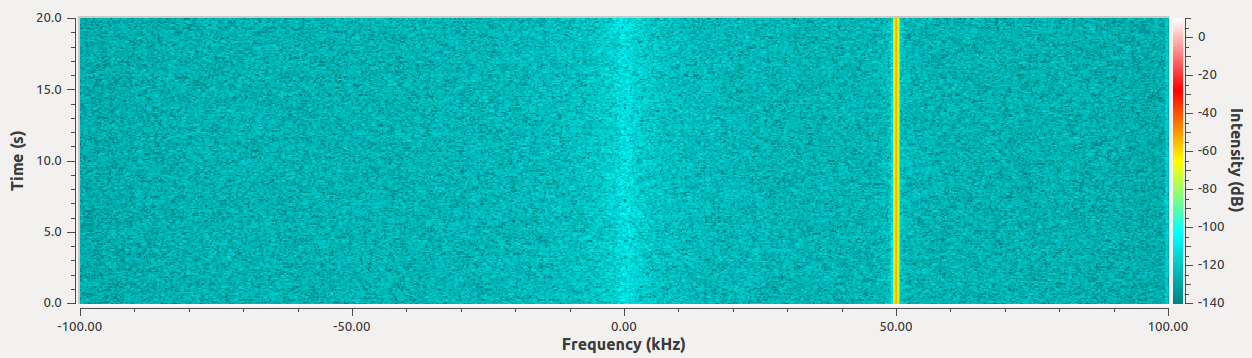
\includegraphics[width=0.9\textwidth]{figures/Spektrum}
        	};
		\begin{scope}[x={(image.south east)},y={(image.north west)}]
		\draw[black,thick,<->] (0.498,0.98) --  node[above, font=\footnotesize] {$\flo = \SI{50}{kHz}$} (0.718,0.98);
		\draw[white, dashed] (0.4,0.155) rectangle node[above, font=\footnotesize, text width = 2cm, align=center] {\textcolor{white}{DC offset and flicker noise}} (0.6,0.942); 

		%\draw[help lines,xstep=.1,ystep=.1] (0,0) grid (1,1);
		%\foreach \x in {0,1,...,9} { \node [anchor=north] at (\x/10,0) {0.\x}; }
		%\foreach \y in {0,1,...,9} { \node [anchor=east] at (0,\y/10) {0.\y}; }
		\end{scope}
		\end{tikzpicture}	
		\label{fig_HVD:SP_os}
	} \\
        \subfloat[Signal after bandpass filtering, filter bandwidth  $= \SI{50}{kHz}$]
	{

		\begin{tikzpicture}[scale=1]
		\node[anchor=south west,inner sep=0] (image) at (0,0)
		{

			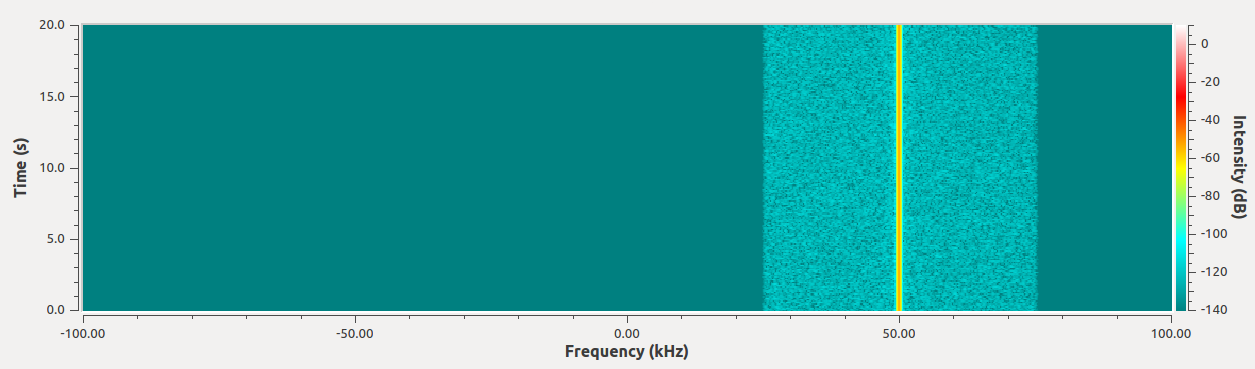
\includegraphics[width=0.9\textwidth]{figures/bpf}
        	};
		\begin{scope}[x={(image.south east)},y={(image.north west)}]
		\draw[black,thick,<->] (0.605,0.98) --  node[above, font=\footnotesize] {Band pass filter = $\SI{50}{kHz}$} (0.825,0.98);

		%\draw[help lines,xstep=.1,ystep=.1] (0,0) grid (1,1);
		%\foreach \x in {0,1,...,9} { \node [anchor=north] at (\x/10,0) {0.\x}; }
		%\foreach \y in {0,1,...,9} { \node [anchor=east] at (0,\y/10) {0.\y}; }
		\end{scope}
		\end{tikzpicture}	
        	\label{fig_HVD:SP_bp}
	} \\
        \subfloat[Signal after digital downconversion]
	{
		
\includegraphics[width=0.9\textwidth]{figures/runtergemischt}
        	\label{fig_HVD:SP_dc}
	} \\
        \subfloat[Signal after decimation]
	{
		
\includegraphics[width=0.9\textwidth]{figures/dezimiert}
        	\label{fig_HVD:SP_de}
	}
        %\vspace{-10 pt}
	\caption{An illustration of the signal processing steps carried out at the host computer to preclude the spurious effects such as the DC offset and the flicker noise on the signal received at the ST.}
        \label{fig_HVD:SP}
\end{figure}


Since the USRP employs a \index{Homodyne receiver}homodyne receiver\footnote{A homodyne receiver implements a direct downconversion of the bandpass to the baseband signal.}, spurious effects such as \index{Spurious effects!DC offset}DC offset, \index{Spurious effects!flicker noise}flicker noise $(1/f)$ and \index{Spurious effects!I/Q imbalance} I/Q imbalance arising from the analog front-end can affect the accuracy of the analytical expressions, thereby influencing the validation process. These spurious effects, particularly the DC offset and the flicker noise, become significant at low signal to noise ratio. In order to retrieve the complex samples close to the one obtained while characterizing the system model that do not take such spurious effects into account, the following signal processing (referred as pre-processing) is proposed at the host computer, please consider \figurename~\ref{fig_HVD:SP}:
\begin{itemize}
\index{Pre-processing!LO-Offset}
\item The received signal is oversampled with sampling frequency of $200$ $\SI{}{kHz}$. 
%Now, for a bandpass filter with bandpass frequency of $\SI{50}{KHz}$ applied subsequently, this sampling corresponds to a oversampling factor = 4. 
In order to filter out the spurious effects\index{Pre-processing}, the local oscillator is tunned at a certain offset frequency defined as $\flo = \SI{50}{kHz}$, refer to \figurename~\ref{fig_HVD:SP_os}. 
\index{Pre-processing!Bandpass filtering}
\item Subsequently, a bandpass filter with bandwidth = $\SI{50}{kHz}$, corresponding to a oversampling factor = $4$, is employed to obtain the desired bandpass signal at the $\flo$. This filters out the DC offset and the flicker noise present at low frequencies, cf. \figurename~\ref{fig_HVD:SP_bp}. 
\index{Pre-processing!digital downconversion}
\item In order to obtain the lowpass equivalent of the desired signal, a digital downconversion (i.e., multiplying with a complex sinusoid with frequency $\flo = \SI{50}{kHz}$) of the bandpass filtered signal is performed, cf. \figurename~\ref{fig_HVD:SP_dc}. %These four steps depicted in \figurename~\ref{fig_HVD:SP} are carried out to remove the receiver's DC offset and the flicker noise (1/f) around the DC. Due to the small bandwidth of the pilot signal, these effects form the bottleneck of our validation and had to be accounted for. 
\index{Pre-processing!decimation}
\item It is worth noticing that the proposed framework considers i.i.d. samples while characterizing the pdfs of the corresponding systems parameters. In this regard, a decimation filter (with decimation factor = 4) over the downconverted signal is applied, cf. \figurename~\ref{fig_HVD:SP_de}, to reduce the correlation between the samples, arising due to oversampling. 
\end{itemize}

\subsection{Determining Noise Power}

\begin{figure}
	%\vspace{-10 pt}
	\centering
	%
\includegraphics[width=0.8\textwidth]{figures/setup}
	  \begin{tikzpicture}[scale=1]
                \node[anchor=south west,inner sep=0] (image) at (0,0)
                {
			\includegraphics[width=0.5\textwidth]{figures/noise_measurement}
                };

                \begin{scope}[x={(image.south east)},y={(image.north west)}]
                \node[draw, fill=gray!10,font=\scriptsize] at (0.59,0.765) {Host Computer};

                \node[draw, fill=gray!10,font=\scriptsize, align = center] at (0.15,0.31) {SDR Platform};
                \node[draw, fill=gray!10,font=\scriptsize, align = center, rotate = 90] at (1.03,0.25) {USB Interface};
                \node[draw, fill=gray!10,font=\scriptsize, align = center] at (0.08,-0.01) {50 $\Omega$ Resistor};
                %\draw[help lines,xstep=.1,ystep=.1] (0,0) grid (1,1);
                %\foreach \x in {0,1,...,9} { \node [anchor=north] at (\x/10,0) {0.\x}; }
                %\foreach \y in {0,1,...,9} { \node [anchor=east] at (0,\y/10) {0.\y}; }
                \end{scope}
        \end{tikzpicture}
	\caption{A measurement setup for acquiring the noise power.}%, consisting of: (i) 50 $\Omega$ resistor connected to the SMA port of the USRP, (ii) Software defined radio platform (USRP B210), (iii) USB interference to the host computer and (iv) host computer.}
	\label{fig_HVD:noise_cal}
	%\vspace{-10 pt}
\end{figure}

Besides these spurious effects, it is challenging to accurately determine the noise power ($\npp$), which is important parameter for characterizing the pdfs. In this regard, $\npp$ is determined using the variance of the envelope of $\yrcvd[n]$ -- \textit{on the fly}. This is done because the value of the noise power evaluated during the calibration (that involves no signal transmission, refer to \figurename~\ref{fig_HVD:noise_cal}) differed from the one determined while performance the measurements for different values of signal to noise ratio ($\snrrcvdu$) received at the ST over the interference channel. It is noticed that the latter approach, presented later in Section \ref{ssec:val_sys}), provided a closer fit to the analytical expressions.


\subsection{Validation of System Parameters}
\index{Hardware validation!system parameters}
\label{ssec:val_sys}
Since the stochastic model is the basis of the proposed analysis, it is reasonable to first validate the pdfs of the system parameters ($\eprcvdstpr$, $\epreg$, $\eprcvdpr$, and $\ers$), derived in Section \ref{model}. To this end, measurements are performed in accordance to the setup, illustrated in \figurename~\ref{messaufbau}. The measurement data is plotted in terms of histogram and scaled to determine the relative frequency ($f_\textrm{hist}(x)$, a discrete function) over a certain set of bins, $x \in \mathcal X_\text{bins}$. \figurename~\ref{hrel_pdf} compares the histograms, obtained from the measurements, and the pdfs, determined using the analytical expressions for a certain set of system parameters depicted in Table \ref{param}. The plots justify the validity of the derived theoretical expressions, which include the pdfs of the system parameters. As a result, these pdfs are eligible for capturing the performance of the CR systems over the hardware. 


\begin{table}
%	\vspace{-10 pt}
	%\setlength{\tabcolsep}{6pt} % spacing between columns
	\renewcommand{\arraystretch}{1.4}
	\centering
	\caption{Values of the parameters determined while performing the experiments.}
	\label{param}
	\begin{tabular}{c||c}
		\bfseries Parameter & \bfseries Value \\ \hline \hline
		$\snrrcvdu$ & \SI{22}{dB} \\
		$N$ & 100 \\
		$\test$ & \SI{2}{ms}\\
		$\ite$ & \SI{-110}{dBm}\\
		$T$ & \SI{100}{ms}\\
		$\pgs$ & 1 \\
		$\npp$ & $\SI{-96.74}{dBm}$\\ \hline
		%Value & \SI{22}{dB} & 100/\SI{0.5}{ms} & \SI{-110}{dBm} & \SI{100]{ms} & 1 \tablefootnote{The channel gain of the ST-SR link $\alpha_\textrm{s} \in (0,1)$ was set to its maximum theoretical value for this analysis.} & $2.1355\times10^{-10}$ \tablefootnote{The value represents the measured receiver noise floor (digital value) of the in-phase or quadrature-phase components.} \\ 
	\end{tabular}
%	%\vspace{-10 pt} 
\end{table}

\begin{figure}
	\vspace{-16 pt}
	\centering
	% This file is generated by the MATLAB m-file laprint.m. It can be included
% into LaTeX documents using the packages graphicx, color and psfrag.
% It is accompanied by a postscript file. A sample LaTeX file is:
%    \documentclass{article}\usepackage{graphicx,color,psfrag}
%    \begin{document}% This file is generated by the MATLAB m-file laprint.m. It can be included
% into LaTeX documents using the packages graphicx, color and psfrag.
% It is accompanied by a postscript file. A sample LaTeX file is:
%    \documentclass{article}\usepackage{graphicx,color,psfrag}
%    \begin{document}% This file is generated by the MATLAB m-file laprint.m. It can be included
% into LaTeX documents using the packages graphicx, color and psfrag.
% It is accompanied by a postscript file. A sample LaTeX file is:
%    \documentclass{article}\usepackage{graphicx,color,psfrag}
%    \begin{document}\input{P_ST_Rx}\end{document}
% See http://www.mathworks.de/matlabcentral/fileexchange/loadFile.do?objectId=4638
% for recent versions of laprint.m.
%
% created by:           LaPrint version 3.16 (13.9.2004)
% created on:           21-Mar-2016 13:21:32
% eps bounding box:     16 cm x 12.0286 cm
% comment:              
%
%\begin{psfrags}%
%\psfragscanon%
%
% text strings:
\psfrag{s05}[t][t]{\fontsize{8}{12}\fontseries{m}\mathversion{normal}\fontshape{n}\selectfont \color[rgb]{0.15,0.15,0.15}\setlength{\tabcolsep}{0pt}\begin{tabular}{c}$\eprcvd$ = [\SI{}{mW}]\end{tabular}}%
\psfrag{s06}[b][b]{\fontsize{8}{12}\fontseries{m}\mathversion{normal}\fontshape{n}\selectfont \color[rgb]{0,0,0}\setlength{\tabcolsep}{0pt}\begin{tabular}{c}pdf\end{tabular}}%
\psfrag{s10}[][]{\fontsize{10}{15}\fontseries{m}\mathversion{normal}\fontshape{n}\selectfont \color[rgb]{0,0,0}\setlength{\tabcolsep}{0pt}\begin{tabular}{c} \end{tabular}}%
\psfrag{s11}[][]{\fontsize{10}{15}\fontseries{m}\mathversion{normal}\fontshape{n}\selectfont \color[rgb]{0,0,0}\setlength{\tabcolsep}{0pt}\begin{tabular}{c} \end{tabular}}%
%\psfrag{s12}[l][l]{\fontsize{8}{12}\fontseries{m}\mathversion{normal}\fontshape{n}\selectfont \color[rgb]{0,0,0}(\ref{eq_HVD:dprcvdstpr})}%
\psfrag{s13}[l][l]{\fontsize{8}{12}\fontseries{m}\mathversion{normal}\fontshape{n}\selectfont \color[rgb]{0,0,0}Empirical}%
\psfrag{s14}[l][l]{\fontsize{8}{12}\fontseries{m}\mathversion{normal}\fontshape{n}\selectfont \color[rgb]{0,0,0}(\ref{eq_HVD:dprcvdstpr})}%
%
% axes font properties:
\fontsize{8}{12}\fontseries{m}\mathversion{normal}%
\fontshape{n}\selectfont%
%
% xticklabels:
\psfrag{x01}[t][t]{3}%
\psfrag{x02}[t][t]{3.2}%
\psfrag{x03}[t][t]{3.4}%
\psfrag{x04}[t][t]{3.6}%
\psfrag{x05}[t][t]{3.8}%
\psfrag{x06}[t][t]{4}%
\psfrag{x07}[t][t]{4.2}%
\psfrag{x08}[t][t]{4.4}%
\psfrag{x09}[t][t]{4.6}%
\psfrag{x10}[t][t]{\shortstack{4.8\\$\times 10^{-9}\ $}}%
%
% yticklabels:
\psfrag{v01}[r][r]{0}%
\psfrag{v02}[r][r]{0.5}%
\psfrag{v03}[r][r]{1}%
\psfrag{v04}[r][r]{1.5}%
\psfrag{v05}[r][r]{2}%
\psfrag{v06}[r][r]{2.5}%
\psfrag{ypower2}[Bl][Bl]{$\times 10^{9}$}%
%
% Figure:
%\resizebox{8cm}{!}{\includegraphics{P_ST_Rx.eps}}%
%\end{psfrags}%
%
% End P_ST_Rx.tex
\end{document}
% See http://www.mathworks.de/matlabcentral/fileexchange/loadFile.do?objectId=4638
% for recent versions of laprint.m.
%
% created by:           LaPrint version 3.16 (13.9.2004)
% created on:           21-Mar-2016 13:21:32
% eps bounding box:     16 cm x 12.0286 cm
% comment:              
%
%\begin{psfrags}%
%\psfragscanon%
%
% text strings:
\psfrag{s05}[t][t]{\fontsize{8}{12}\fontseries{m}\mathversion{normal}\fontshape{n}\selectfont \color[rgb]{0.15,0.15,0.15}\setlength{\tabcolsep}{0pt}\begin{tabular}{c}$\eprcvd$ = [\SI{}{mW}]\end{tabular}}%
\psfrag{s06}[b][b]{\fontsize{8}{12}\fontseries{m}\mathversion{normal}\fontshape{n}\selectfont \color[rgb]{0,0,0}\setlength{\tabcolsep}{0pt}\begin{tabular}{c}pdf\end{tabular}}%
\psfrag{s10}[][]{\fontsize{10}{15}\fontseries{m}\mathversion{normal}\fontshape{n}\selectfont \color[rgb]{0,0,0}\setlength{\tabcolsep}{0pt}\begin{tabular}{c} \end{tabular}}%
\psfrag{s11}[][]{\fontsize{10}{15}\fontseries{m}\mathversion{normal}\fontshape{n}\selectfont \color[rgb]{0,0,0}\setlength{\tabcolsep}{0pt}\begin{tabular}{c} \end{tabular}}%
%\psfrag{s12}[l][l]{\fontsize{8}{12}\fontseries{m}\mathversion{normal}\fontshape{n}\selectfont \color[rgb]{0,0,0}(\ref{eq_HVD:dprcvdstpr})}%
\psfrag{s13}[l][l]{\fontsize{8}{12}\fontseries{m}\mathversion{normal}\fontshape{n}\selectfont \color[rgb]{0,0,0}Empirical}%
\psfrag{s14}[l][l]{\fontsize{8}{12}\fontseries{m}\mathversion{normal}\fontshape{n}\selectfont \color[rgb]{0,0,0}(\ref{eq_HVD:dprcvdstpr})}%
%
% axes font properties:
\fontsize{8}{12}\fontseries{m}\mathversion{normal}%
\fontshape{n}\selectfont%
%
% xticklabels:
\psfrag{x01}[t][t]{3}%
\psfrag{x02}[t][t]{3.2}%
\psfrag{x03}[t][t]{3.4}%
\psfrag{x04}[t][t]{3.6}%
\psfrag{x05}[t][t]{3.8}%
\psfrag{x06}[t][t]{4}%
\psfrag{x07}[t][t]{4.2}%
\psfrag{x08}[t][t]{4.4}%
\psfrag{x09}[t][t]{4.6}%
\psfrag{x10}[t][t]{\shortstack{4.8\\$\times 10^{-9}\ $}}%
%
% yticklabels:
\psfrag{v01}[r][r]{0}%
\psfrag{v02}[r][r]{0.5}%
\psfrag{v03}[r][r]{1}%
\psfrag{v04}[r][r]{1.5}%
\psfrag{v05}[r][r]{2}%
\psfrag{v06}[r][r]{2.5}%
\psfrag{ypower2}[Bl][Bl]{$\times 10^{9}$}%
%
% Figure:
%\resizebox{8cm}{!}{\includegraphics{P_ST_Rx.eps}}%
%\end{psfrags}%
%
% End P_ST_Rx.tex
\end{document}
% See http://www.mathworks.de/matlabcentral/fileexchange/loadFile.do?objectId=4638
% for recent versions of laprint.m.
%
% created by:           LaPrint version 3.16 (13.9.2004)
% created on:           21-Mar-2016 13:21:32
% eps bounding box:     16 cm x 12.0286 cm
% comment:              
%
%\begin{psfrags}%
%\psfragscanon%
%
% text strings:
\psfrag{s05}[t][t]{\fontsize{8}{12}\fontseries{m}\mathversion{normal}\fontshape{n}\selectfont \color[rgb]{0.15,0.15,0.15}\setlength{\tabcolsep}{0pt}\begin{tabular}{c}$\eprcvd$ = [\SI{}{mW}]\end{tabular}}%
\psfrag{s06}[b][b]{\fontsize{8}{12}\fontseries{m}\mathversion{normal}\fontshape{n}\selectfont \color[rgb]{0,0,0}\setlength{\tabcolsep}{0pt}\begin{tabular}{c}pdf\end{tabular}}%
\psfrag{s10}[][]{\fontsize{10}{15}\fontseries{m}\mathversion{normal}\fontshape{n}\selectfont \color[rgb]{0,0,0}\setlength{\tabcolsep}{0pt}\begin{tabular}{c} \end{tabular}}%
\psfrag{s11}[][]{\fontsize{10}{15}\fontseries{m}\mathversion{normal}\fontshape{n}\selectfont \color[rgb]{0,0,0}\setlength{\tabcolsep}{0pt}\begin{tabular}{c} \end{tabular}}%
%\psfrag{s12}[l][l]{\fontsize{8}{12}\fontseries{m}\mathversion{normal}\fontshape{n}\selectfont \color[rgb]{0,0,0}(\ref{eq_HVD:dprcvdstpr})}%
\psfrag{s13}[l][l]{\fontsize{8}{12}\fontseries{m}\mathversion{normal}\fontshape{n}\selectfont \color[rgb]{0,0,0}Empirical}%
\psfrag{s14}[l][l]{\fontsize{8}{12}\fontseries{m}\mathversion{normal}\fontshape{n}\selectfont \color[rgb]{0,0,0}(\ref{eq_HVD:dprcvdstpr})}%
%
% axes font properties:
\fontsize{8}{12}\fontseries{m}\mathversion{normal}%
\fontshape{n}\selectfont%
%
% xticklabels:
\psfrag{x01}[t][t]{3}%
\psfrag{x02}[t][t]{3.2}%
\psfrag{x03}[t][t]{3.4}%
\psfrag{x04}[t][t]{3.6}%
\psfrag{x05}[t][t]{3.8}%
\psfrag{x06}[t][t]{4}%
\psfrag{x07}[t][t]{4.2}%
\psfrag{x08}[t][t]{4.4}%
\psfrag{x09}[t][t]{4.6}%
\psfrag{x10}[t][t]{\shortstack{4.8\\$\times 10^{-9}\ $}}%
%
% yticklabels:
\psfrag{v01}[r][r]{0}%
\psfrag{v02}[r][r]{0.5}%
\psfrag{v03}[r][r]{1}%
\psfrag{v04}[r][r]{1.5}%
\psfrag{v05}[r][r]{2}%
\psfrag{v06}[r][r]{2.5}%
\psfrag{ypower2}[Bl][Bl]{$\times 10^{9}$}%
%
% Figure:
%\resizebox{8cm}{!}{\includegraphics{P_ST_Rx.eps}}%
%\end{psfrags}%
%
% End P_ST_Rx.tex

	\begin{tikzpicture}[scale=1]
                \node[anchor=south west,inner sep=0] (image) at (0,0)
        	{
			\includegraphics[width=0.52\textwidth]{figures/P_ST_Rx} 
                };

		\begin{scope}[x={(image.south east)},y={(image.north west)}]
                \node[above, font=\footnotesize] at (0.16,0.93) {$ \times 10^{-9}$};

                %\draw[help lines,xstep=.1,ystep=.1] (0,0) grid (1,1);
                %\foreach \x in {0,1,...,9} { \node [anchor=north] at (\x/10,0) {0.\x}; }
                %\foreach \y in {0,1,...,9} { \node [anchor=east] at (0,\y/10) {0.\y}; }
                \end{scope}
        \end{tikzpicture}\\[5pt] %

	
	% This file is generated by the MATLAB m-file laprint.m. It can be included
% into LaTeX documents using the packages graphicx, color and psfrag.
% It is accompanied by a postscript file. A sample LaTeX file is:
%    \documentclass{article}\usepackage{graphicx,color,psfrag}
%    \begin{document}% This file is generated by the MATLAB m-file laprint.m. It can be included
% into LaTeX documents using the packages graphicx, color and psfrag.
% It is accompanied by a postscript file. A sample LaTeX file is:
%    \documentclass{article}\usepackage{graphicx,color,psfrag}
%    \begin{document}% This file is generated by the MATLAB m-file laprint.m. It can be included
% into LaTeX documents using the packages graphicx, color and psfrag.
% It is accompanied by a postscript file. A sample LaTeX file is:
%    \documentclass{article}\usepackage{graphicx,color,psfrag}
%    \begin{document}\input{P_ST_Tx}\end{document}
% See http://www.mathworks.de/matlabcentral/fileexchange/loadFile.do?objectId=4638
% for recent versions of laprint.m.
%
% created by:           LaPrint version 3.16 (13.9.2004)
% created on:           21-Mar-2016 13:19:58
% eps bounding box:     16 cm x 12 cm
% comment:              
%
%\begin{psfrags}%
%\psfragscanon%
%
% text strings:
\psfrag{s05}[t][t]{\fontsize{8}{12}\fontseries{m}\mathversion{normal}\fontshape{n}\selectfont \color[rgb]{0.15,0.15,0.15}\setlength{\tabcolsep}{0pt}\begin{tabular}{c}$\epreg$ = [dBm]\end{tabular}}%
\psfrag{s06}[b][b]{\fontsize{8}{12}\fontseries{m}\mathversion{normal}\fontshape{n}\selectfont \color[rgb]{0,0,0}\setlength{\tabcolsep}{0pt}\begin{tabular}{c}pdf\end{tabular}}%
\psfrag{s10}[][]{\fontsize{10}{15}\fontseries{m}\mathversion{normal}\fontshape{n}\selectfont \color[rgb]{0,0,0}\setlength{\tabcolsep}{0pt}\begin{tabular}{c} \end{tabular}}%
\psfrag{s11}[][]{\fontsize{10}{15}\fontseries{m}\mathversion{normal}\fontshape{n}\selectfont \color[rgb]{0,0,0}\setlength{\tabcolsep}{0pt}\begin{tabular}{c} \end{tabular}}%
%\psfrag{s12}[l][l]{\fontsize{8}{12}\fontseries{m}\mathversion{normal}\fontshape{n}\selectfont \color[rgb]{0,0,0}(\ref{eq_HVD:dpreg})}%
\psfrag{s13}[l][l]{\fontsize{8}{12}\fontseries{m}\mathversion{normal}\fontshape{n}\selectfont \color[rgb]{0,0,0}Empirical}%
\psfrag{s14}[l][l]{\fontsize{8}{12}\fontseries{m}\mathversion{normal}\fontshape{n}\selectfont \color[rgb]{0,0,0}(\ref{eq_HVD:dpreg})}%
%
% axes font properties:
\fontsize{8}{12}\fontseries{m}\mathversion{normal}%
\fontshape{n}\selectfont%
%
% xticklabels:
\psfrag{x01}[t][t]{2.2}%
\psfrag{x02}[t][t]{2.4}%
\psfrag{x03}[t][t]{2.6}%
\psfrag{x04}[t][t]{2.8}%
\psfrag{x05}[t][t]{3}%
\psfrag{x06}[t][t]{3.2}%
\psfrag{x07}[t][t]{\shortstack{3.4\\$\times 10^{-8}\ $}}%
%
% yticklabels:
\psfrag{v01}[r][r]{0}%
\psfrag{v02}[r][r]{0.5}%
\psfrag{v03}[r][r]{1}%
\psfrag{v04}[r][r]{1.5}%
\psfrag{v05}[r][r]{2}%
\psfrag{v06}[r][r]{2.5}%
\psfrag{v07}[r][r]{3}%
\psfrag{v08}[r][r]{3.5}%
\psfrag{ypower2}[Bl][Bl]{$\times 10^{8}$}%
%
% Figure:
%\resizebox{8cm}{!}{\includegraphics{P_ST_Tx.eps}}%
%\end{psfrags}%
%
% End P_ST_Tx.tex
\end{document}
% See http://www.mathworks.de/matlabcentral/fileexchange/loadFile.do?objectId=4638
% for recent versions of laprint.m.
%
% created by:           LaPrint version 3.16 (13.9.2004)
% created on:           21-Mar-2016 13:19:58
% eps bounding box:     16 cm x 12 cm
% comment:              
%
%\begin{psfrags}%
%\psfragscanon%
%
% text strings:
\psfrag{s05}[t][t]{\fontsize{8}{12}\fontseries{m}\mathversion{normal}\fontshape{n}\selectfont \color[rgb]{0.15,0.15,0.15}\setlength{\tabcolsep}{0pt}\begin{tabular}{c}$\epreg$ = [dBm]\end{tabular}}%
\psfrag{s06}[b][b]{\fontsize{8}{12}\fontseries{m}\mathversion{normal}\fontshape{n}\selectfont \color[rgb]{0,0,0}\setlength{\tabcolsep}{0pt}\begin{tabular}{c}pdf\end{tabular}}%
\psfrag{s10}[][]{\fontsize{10}{15}\fontseries{m}\mathversion{normal}\fontshape{n}\selectfont \color[rgb]{0,0,0}\setlength{\tabcolsep}{0pt}\begin{tabular}{c} \end{tabular}}%
\psfrag{s11}[][]{\fontsize{10}{15}\fontseries{m}\mathversion{normal}\fontshape{n}\selectfont \color[rgb]{0,0,0}\setlength{\tabcolsep}{0pt}\begin{tabular}{c} \end{tabular}}%
%\psfrag{s12}[l][l]{\fontsize{8}{12}\fontseries{m}\mathversion{normal}\fontshape{n}\selectfont \color[rgb]{0,0,0}(\ref{eq_HVD:dpreg})}%
\psfrag{s13}[l][l]{\fontsize{8}{12}\fontseries{m}\mathversion{normal}\fontshape{n}\selectfont \color[rgb]{0,0,0}Empirical}%
\psfrag{s14}[l][l]{\fontsize{8}{12}\fontseries{m}\mathversion{normal}\fontshape{n}\selectfont \color[rgb]{0,0,0}(\ref{eq_HVD:dpreg})}%
%
% axes font properties:
\fontsize{8}{12}\fontseries{m}\mathversion{normal}%
\fontshape{n}\selectfont%
%
% xticklabels:
\psfrag{x01}[t][t]{2.2}%
\psfrag{x02}[t][t]{2.4}%
\psfrag{x03}[t][t]{2.6}%
\psfrag{x04}[t][t]{2.8}%
\psfrag{x05}[t][t]{3}%
\psfrag{x06}[t][t]{3.2}%
\psfrag{x07}[t][t]{\shortstack{3.4\\$\times 10^{-8}\ $}}%
%
% yticklabels:
\psfrag{v01}[r][r]{0}%
\psfrag{v02}[r][r]{0.5}%
\psfrag{v03}[r][r]{1}%
\psfrag{v04}[r][r]{1.5}%
\psfrag{v05}[r][r]{2}%
\psfrag{v06}[r][r]{2.5}%
\psfrag{v07}[r][r]{3}%
\psfrag{v08}[r][r]{3.5}%
\psfrag{ypower2}[Bl][Bl]{$\times 10^{8}$}%
%
% Figure:
%\resizebox{8cm}{!}{\includegraphics{P_ST_Tx.eps}}%
%\end{psfrags}%
%
% End P_ST_Tx.tex
\end{document}
% See http://www.mathworks.de/matlabcentral/fileexchange/loadFile.do?objectId=4638
% for recent versions of laprint.m.
%
% created by:           LaPrint version 3.16 (13.9.2004)
% created on:           21-Mar-2016 13:19:58
% eps bounding box:     16 cm x 12 cm
% comment:              
%
%\begin{psfrags}%
%\psfragscanon%
%
% text strings:
\psfrag{s05}[t][t]{\fontsize{8}{12}\fontseries{m}\mathversion{normal}\fontshape{n}\selectfont \color[rgb]{0.15,0.15,0.15}\setlength{\tabcolsep}{0pt}\begin{tabular}{c}$\epreg$ = [dBm]\end{tabular}}%
\psfrag{s06}[b][b]{\fontsize{8}{12}\fontseries{m}\mathversion{normal}\fontshape{n}\selectfont \color[rgb]{0,0,0}\setlength{\tabcolsep}{0pt}\begin{tabular}{c}pdf\end{tabular}}%
\psfrag{s10}[][]{\fontsize{10}{15}\fontseries{m}\mathversion{normal}\fontshape{n}\selectfont \color[rgb]{0,0,0}\setlength{\tabcolsep}{0pt}\begin{tabular}{c} \end{tabular}}%
\psfrag{s11}[][]{\fontsize{10}{15}\fontseries{m}\mathversion{normal}\fontshape{n}\selectfont \color[rgb]{0,0,0}\setlength{\tabcolsep}{0pt}\begin{tabular}{c} \end{tabular}}%
%\psfrag{s12}[l][l]{\fontsize{8}{12}\fontseries{m}\mathversion{normal}\fontshape{n}\selectfont \color[rgb]{0,0,0}(\ref{eq_HVD:dpreg})}%
\psfrag{s13}[l][l]{\fontsize{8}{12}\fontseries{m}\mathversion{normal}\fontshape{n}\selectfont \color[rgb]{0,0,0}Empirical}%
\psfrag{s14}[l][l]{\fontsize{8}{12}\fontseries{m}\mathversion{normal}\fontshape{n}\selectfont \color[rgb]{0,0,0}(\ref{eq_HVD:dpreg})}%
%
% axes font properties:
\fontsize{8}{12}\fontseries{m}\mathversion{normal}%
\fontshape{n}\selectfont%
%
% xticklabels:
\psfrag{x01}[t][t]{2.2}%
\psfrag{x02}[t][t]{2.4}%
\psfrag{x03}[t][t]{2.6}%
\psfrag{x04}[t][t]{2.8}%
\psfrag{x05}[t][t]{3}%
\psfrag{x06}[t][t]{3.2}%
\psfrag{x07}[t][t]{\shortstack{3.4\\$\times 10^{-8}\ $}}%
%
% yticklabels:
\psfrag{v01}[r][r]{0}%
\psfrag{v02}[r][r]{0.5}%
\psfrag{v03}[r][r]{1}%
\psfrag{v04}[r][r]{1.5}%
\psfrag{v05}[r][r]{2}%
\psfrag{v06}[r][r]{2.5}%
\psfrag{v07}[r][r]{3}%
\psfrag{v08}[r][r]{3.5}%
\psfrag{ypower2}[Bl][Bl]{$\times 10^{8}$}%
%
% Figure:
%\resizebox{8cm}{!}{\includegraphics{P_ST_Tx.eps}}%
%\end{psfrags}%
%
% End P_ST_Tx.tex

	\begin{tikzpicture}[scale=1]
                \node[anchor=south west,inner sep=0] (image) at (0,0)
        	{
			\includegraphics[width=0.52\textwidth]{figures/P_ST_Tx} 
                };

		\begin{scope}[x={(image.south east)},y={(image.north west)}]
                \node[above, font=\footnotesize] at (0.16,0.93) {$ \times 10^{-8}$};

                %\draw[help lines,xstep=.1,ystep=.1] (0,0) grid (1,1);
                %\foreach \x in {0,1,...,9} { \node [anchor=north] at (\x/10,0) {0.\x}; }
                %\foreach \y in {0,1,...,9} { \node [anchor=east] at (0,\y/10) {0.\y}; }
                \end{scope}
        \end{tikzpicture}\\[5pt] %

	
	% This file is generated by the MATLAB m-file laprint.m. It can be included
% into LaTeX documents using the packages graphicx, color and psfrag.
% It is accompanied by a postscript file. A sample LaTeX file is:
%    \documentclass{article}\usepackage{graphicx,color,psfrag}
%    \begin{document}% This file is generated by the MATLAB m-file laprint.m. It can be included
% into LaTeX documents using the packages graphicx, color and psfrag.
% It is accompanied by a postscript file. A sample LaTeX file is:
%    \documentclass{article}\usepackage{graphicx,color,psfrag}
%    \begin{document}% This file is generated by the MATLAB m-file laprint.m. It can be included
% into LaTeX documents using the packages graphicx, color and psfrag.
% It is accompanied by a postscript file. A sample LaTeX file is:
%    \documentclass{article}\usepackage{graphicx,color,psfrag}
%    \begin{document}\input{P_PR_Rx}\end{document}
% See http://www.mathworks.de/matlabcentral/fileexchange/loadFile.do?objectId=4638
% for recent versions of laprint.m.
%
% created by:           LaPrint version 3.16 (13.9.2004)
% created on:           21-Mar-2016 13:19:59
% eps bounding box:     16 cm x 12.1449 cm
% comment:              
%
%\begin{psfrags}%
%\psfragscanon%
%
% text strings:
\psfrag{s05}[t][t]{\fontsize{8}{12}\fontseries{m}\mathversion{normal}\fontshape{n}\selectfont \color[rgb]{0.15,0.15,0.15}\setlength{\tabcolsep}{0pt}\begin{tabular}{c}$\eprcvdpr$ = [dBm]\end{tabular}}%
\psfrag{s06}[b][b]{\fontsize{8}{12}\fontseries{m}\mathversion{normal}\fontshape{n}\selectfont \color[rgb]{0,0,0}\setlength{\tabcolsep}{0pt}\begin{tabular}{c}pdf\end{tabular}}%
\psfrag{s10}[][]{\fontsize{10}{15}\fontseries{m}\mathversion{normal}\fontshape{n}\selectfont \color[rgb]{0,0,0}\setlength{\tabcolsep}{0pt}\begin{tabular}{c} \end{tabular}}%
\psfrag{s11}[][]{\fontsize{10}{15}\fontseries{m}\mathversion{normal}\fontshape{n}\selectfont \color[rgb]{0,0,0}\setlength{\tabcolsep}{0pt}\begin{tabular}{c} \end{tabular}}%
%\psfrag{s12}[l][l]{\fontsize{8}{12}\fontseries{m}\mathversion{normal}\fontshape{n}\selectfont \color[rgb]{0,0,0}(\ref{eq_HVD:dpp})}%
\psfrag{s13}[l][l]{\fontsize{8}{12}\fontseries{m}\mathversion{normal}\fontshape{n}\selectfont \color[rgb]{0,0,0}Empirical}%
\psfrag{s14}[l][l]{\fontsize{8}{12}\fontseries{m}\mathversion{normal}\fontshape{n}\selectfont \color[rgb]{0,0,0}(\ref{eq_HVD:dpp})}%
%
% axes font properties:
\fontsize{8}{12}\fontseries{m}\mathversion{normal}%
\fontshape{n}\selectfont%
%
% xticklabels:
\psfrag{x01}[t][t]{0.8}%
\psfrag{x02}[t][t]{0.85}%
\psfrag{x03}[t][t]{0.9}%
\psfrag{x04}[t][t]{0.95}%
\psfrag{x05}[t][t]{1}%
\psfrag{x06}[t][t]{1.05}%
\psfrag{x07}[t][t]{1.1}%
\psfrag{x08}[t][t]{1.15}%
\psfrag{x09}[t][t]{1.2}%
\psfrag{x10}[t][t]{\shortstack{1.25\\$\times 10^{-11}\ $}}%
%
% yticklabels:
\psfrag{v01}[r][r]{0}%
\psfrag{v02}[r][r]{1}%
\psfrag{v03}[r][r]{2}%
\psfrag{v04}[r][r]{3}%
\psfrag{v05}[r][r]{4}%
\psfrag{v06}[r][r]{5}%
\psfrag{v07}[r][r]{6}%
\psfrag{v08}[r][r]{7}%
\psfrag{v09}[r][r]{8}%
\psfrag{v10}[r][r]{9}%
\psfrag{v11}[r][r]{10}%
\psfrag{ypower2}[Bl][Bl]{$\times 10^{11}$}%
%
% Figure:
%\resizebox{8cm}{!}{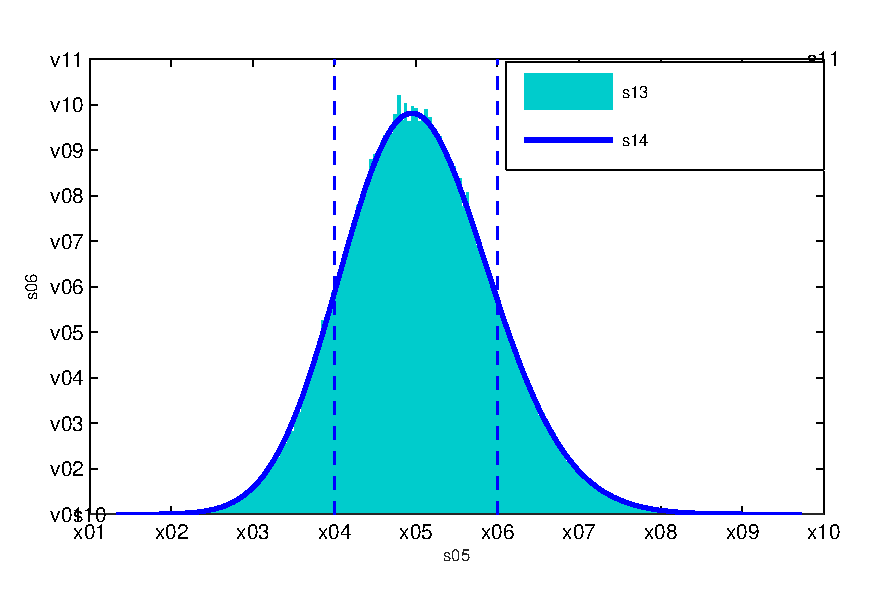
\includegraphics{P_PR_Rx.eps}}%
%\end{psfrags}%
%
% End P_PR_Rx.tex
\end{document}
% See http://www.mathworks.de/matlabcentral/fileexchange/loadFile.do?objectId=4638
% for recent versions of laprint.m.
%
% created by:           LaPrint version 3.16 (13.9.2004)
% created on:           21-Mar-2016 13:19:59
% eps bounding box:     16 cm x 12.1449 cm
% comment:              
%
%\begin{psfrags}%
%\psfragscanon%
%
% text strings:
\psfrag{s05}[t][t]{\fontsize{8}{12}\fontseries{m}\mathversion{normal}\fontshape{n}\selectfont \color[rgb]{0.15,0.15,0.15}\setlength{\tabcolsep}{0pt}\begin{tabular}{c}$\eprcvdpr$ = [dBm]\end{tabular}}%
\psfrag{s06}[b][b]{\fontsize{8}{12}\fontseries{m}\mathversion{normal}\fontshape{n}\selectfont \color[rgb]{0,0,0}\setlength{\tabcolsep}{0pt}\begin{tabular}{c}pdf\end{tabular}}%
\psfrag{s10}[][]{\fontsize{10}{15}\fontseries{m}\mathversion{normal}\fontshape{n}\selectfont \color[rgb]{0,0,0}\setlength{\tabcolsep}{0pt}\begin{tabular}{c} \end{tabular}}%
\psfrag{s11}[][]{\fontsize{10}{15}\fontseries{m}\mathversion{normal}\fontshape{n}\selectfont \color[rgb]{0,0,0}\setlength{\tabcolsep}{0pt}\begin{tabular}{c} \end{tabular}}%
%\psfrag{s12}[l][l]{\fontsize{8}{12}\fontseries{m}\mathversion{normal}\fontshape{n}\selectfont \color[rgb]{0,0,0}(\ref{eq_HVD:dpp})}%
\psfrag{s13}[l][l]{\fontsize{8}{12}\fontseries{m}\mathversion{normal}\fontshape{n}\selectfont \color[rgb]{0,0,0}Empirical}%
\psfrag{s14}[l][l]{\fontsize{8}{12}\fontseries{m}\mathversion{normal}\fontshape{n}\selectfont \color[rgb]{0,0,0}(\ref{eq_HVD:dpp})}%
%
% axes font properties:
\fontsize{8}{12}\fontseries{m}\mathversion{normal}%
\fontshape{n}\selectfont%
%
% xticklabels:
\psfrag{x01}[t][t]{0.8}%
\psfrag{x02}[t][t]{0.85}%
\psfrag{x03}[t][t]{0.9}%
\psfrag{x04}[t][t]{0.95}%
\psfrag{x05}[t][t]{1}%
\psfrag{x06}[t][t]{1.05}%
\psfrag{x07}[t][t]{1.1}%
\psfrag{x08}[t][t]{1.15}%
\psfrag{x09}[t][t]{1.2}%
\psfrag{x10}[t][t]{\shortstack{1.25\\$\times 10^{-11}\ $}}%
%
% yticklabels:
\psfrag{v01}[r][r]{0}%
\psfrag{v02}[r][r]{1}%
\psfrag{v03}[r][r]{2}%
\psfrag{v04}[r][r]{3}%
\psfrag{v05}[r][r]{4}%
\psfrag{v06}[r][r]{5}%
\psfrag{v07}[r][r]{6}%
\psfrag{v08}[r][r]{7}%
\psfrag{v09}[r][r]{8}%
\psfrag{v10}[r][r]{9}%
\psfrag{v11}[r][r]{10}%
\psfrag{ypower2}[Bl][Bl]{$\times 10^{11}$}%
%
% Figure:
%\resizebox{8cm}{!}{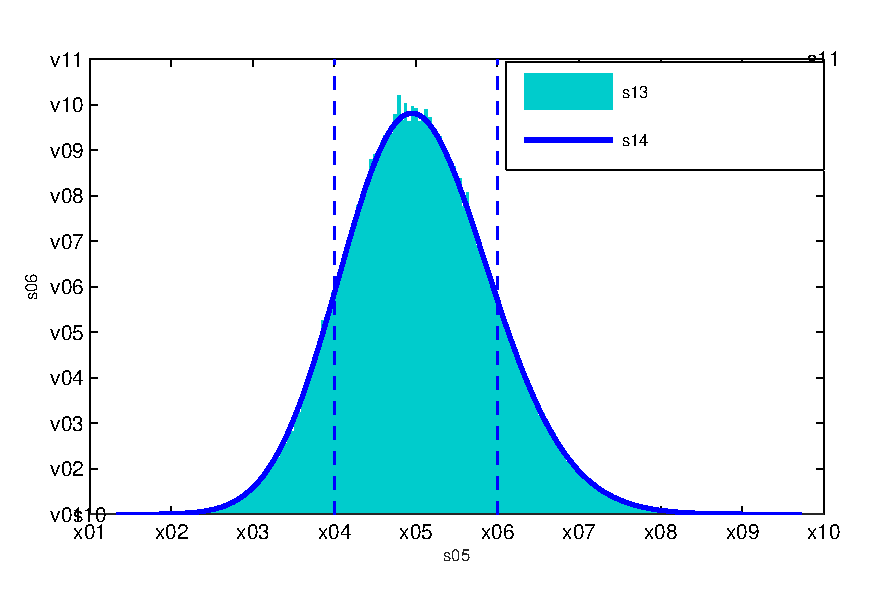
\includegraphics{P_PR_Rx.eps}}%
%\end{psfrags}%
%
% End P_PR_Rx.tex
\end{document}
% See http://www.mathworks.de/matlabcentral/fileexchange/loadFile.do?objectId=4638
% for recent versions of laprint.m.
%
% created by:           LaPrint version 3.16 (13.9.2004)
% created on:           21-Mar-2016 13:19:59
% eps bounding box:     16 cm x 12.1449 cm
% comment:              
%
%\begin{psfrags}%
%\psfragscanon%
%
% text strings:
\psfrag{s05}[t][t]{\fontsize{8}{12}\fontseries{m}\mathversion{normal}\fontshape{n}\selectfont \color[rgb]{0.15,0.15,0.15}\setlength{\tabcolsep}{0pt}\begin{tabular}{c}$\eprcvdpr$ = [dBm]\end{tabular}}%
\psfrag{s06}[b][b]{\fontsize{8}{12}\fontseries{m}\mathversion{normal}\fontshape{n}\selectfont \color[rgb]{0,0,0}\setlength{\tabcolsep}{0pt}\begin{tabular}{c}pdf\end{tabular}}%
\psfrag{s10}[][]{\fontsize{10}{15}\fontseries{m}\mathversion{normal}\fontshape{n}\selectfont \color[rgb]{0,0,0}\setlength{\tabcolsep}{0pt}\begin{tabular}{c} \end{tabular}}%
\psfrag{s11}[][]{\fontsize{10}{15}\fontseries{m}\mathversion{normal}\fontshape{n}\selectfont \color[rgb]{0,0,0}\setlength{\tabcolsep}{0pt}\begin{tabular}{c} \end{tabular}}%
%\psfrag{s12}[l][l]{\fontsize{8}{12}\fontseries{m}\mathversion{normal}\fontshape{n}\selectfont \color[rgb]{0,0,0}(\ref{eq_HVD:dpp})}%
\psfrag{s13}[l][l]{\fontsize{8}{12}\fontseries{m}\mathversion{normal}\fontshape{n}\selectfont \color[rgb]{0,0,0}Empirical}%
\psfrag{s14}[l][l]{\fontsize{8}{12}\fontseries{m}\mathversion{normal}\fontshape{n}\selectfont \color[rgb]{0,0,0}(\ref{eq_HVD:dpp})}%
%
% axes font properties:
\fontsize{8}{12}\fontseries{m}\mathversion{normal}%
\fontshape{n}\selectfont%
%
% xticklabels:
\psfrag{x01}[t][t]{0.8}%
\psfrag{x02}[t][t]{0.85}%
\psfrag{x03}[t][t]{0.9}%
\psfrag{x04}[t][t]{0.95}%
\psfrag{x05}[t][t]{1}%
\psfrag{x06}[t][t]{1.05}%
\psfrag{x07}[t][t]{1.1}%
\psfrag{x08}[t][t]{1.15}%
\psfrag{x09}[t][t]{1.2}%
\psfrag{x10}[t][t]{\shortstack{1.25\\$\times 10^{-11}\ $}}%
%
% yticklabels:
\psfrag{v01}[r][r]{0}%
\psfrag{v02}[r][r]{1}%
\psfrag{v03}[r][r]{2}%
\psfrag{v04}[r][r]{3}%
\psfrag{v05}[r][r]{4}%
\psfrag{v06}[r][r]{5}%
\psfrag{v07}[r][r]{6}%
\psfrag{v08}[r][r]{7}%
\psfrag{v09}[r][r]{8}%
\psfrag{v10}[r][r]{9}%
\psfrag{v11}[r][r]{10}%
\psfrag{ypower2}[Bl][Bl]{$\times 10^{11}$}%
%
% Figure:
%\resizebox{8cm}{!}{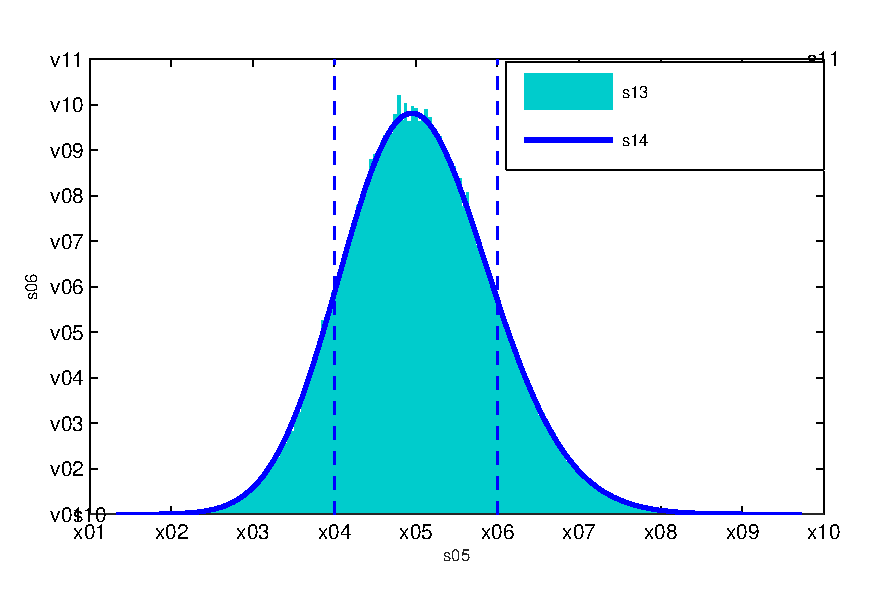
\includegraphics{P_PR_Rx.eps}}%
%\end{psfrags}%
%
% End P_PR_Rx.tex

	\begin{tikzpicture}[scale=1]
                \node[anchor=south west,inner sep=0] (image) at (0,0)
        	{
			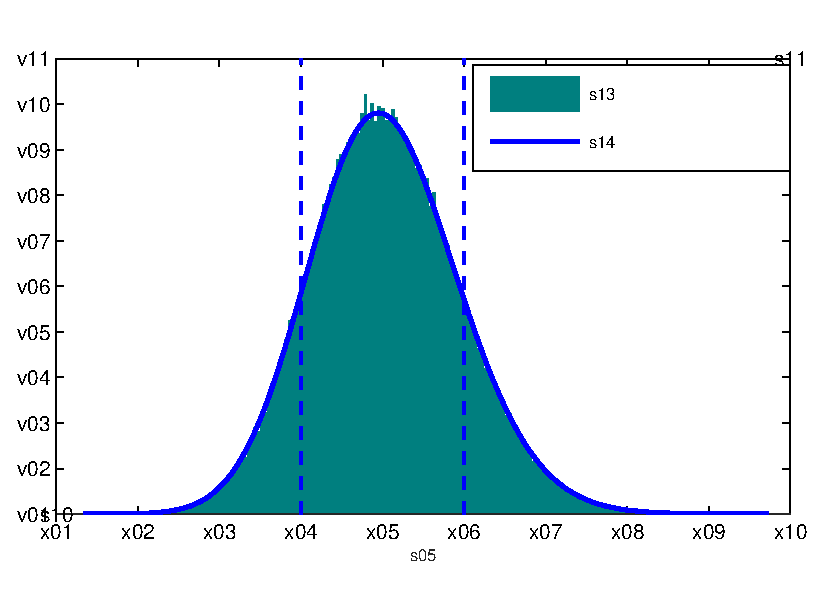
\includegraphics[width=0.52\textwidth]{figures/P_PR_Rx} 
                };

		\begin{scope}[x={(image.south east)},y={(image.north west)}]
                \node[above, font=\footnotesize] at (0.16,0.93) {$ \times 10^{-11}$};

		\draw[black,thick,<-] (0.577,0.57) --  node[above, font=\footnotesize] {$\ite (1 + \acc)$} (0.777,0.57);
		\draw[black,thick,<-] (0.379,0.57) --  node[above, font=\footnotesize] {$\ite (1 - \acc)$} (0.179,0.57);
                %\draw[help lines,xstep=.1,ystep=.1] (0,0) grid (1,1);
                %\foreach \x in {0,1,...,9} { \node [anchor=north] at (\x/10,0) {0.\x}; }
                %\foreach \y in {0,1,...,9} { \node [anchor=east] at (0,\y/10) {0.\y}; }
                \end{scope}
        \end{tikzpicture}\\[10pt] %

	% This file is generated by the MATLAB m-file laprint.m. It can be included
% into LaTeX documents using the packages graphicx, color and psfrag.
% It is accompanied by a postscript file. A sample LaTeX file is:
%    \documentclass{article}\usepackage{graphicx,color,psfrag}
%    \begin{document}% This file is generated by the MATLAB m-file laprint.m. It can be included
% into LaTeX documents using the packages graphicx, color and psfrag.
% It is accompanied by a postscript file. A sample LaTeX file is:
%    \documentclass{article}\usepackage{graphicx,color,psfrag}
%    \begin{document}% This file is generated by the MATLAB m-file laprint.m. It can be included
% into LaTeX documents using the packages graphicx, color and psfrag.
% It is accompanied by a postscript file. A sample LaTeX file is:
%    \documentclass{article}\usepackage{graphicx,color,psfrag}
%    \begin{document}\input{R_s}\end{document}
% See http://www.mathworks.de/matlabcentral/fileexchange/loadFile.do?objectId=4638
% for recent versions of laprint.m.
%
% created by:           LaPrint version 3.16 (13.9.2004)
% created on:           21-Mar-2016 13:20:00
% eps bounding box:     16 cm x 12.1449 cm
% comment:              
%
%\begin{psfrags}%
%\psfragscanon%
%
% text strings:
\psfrag{s05}[t][t]{\fontsize{8}{12}\fontseries{m}\mathversion{normal}\fontshape{n}\selectfont \color[rgb]{0.15,0.15,0.15}\setlength{\tabcolsep}{0pt}\begin{tabular}{c}$\ers$ [bits/sec/Hz]\end{tabular}}%
\psfrag{s06}[b][b]{\fontsize{8}{12}\fontseries{m}\mathversion{normal}\fontshape{n}\selectfont \color[rgb]{0,0,0}\setlength{\tabcolsep}{0pt}\begin{tabular}{c}pdf\end{tabular}}%
\psfrag{s10}[][]{\fontsize{10}{15}\fontseries{m}\mathversion{normal}\fontshape{n}\selectfont \color[rgb]{0,0,0}\setlength{\tabcolsep}{0pt}\begin{tabular}{c} \end{tabular}}%
\psfrag{s11}[][]{\fontsize{10}{15}\fontseries{m}\mathversion{normal}\fontshape{n}\selectfont \color[rgb]{0,0,0}\setlength{\tabcolsep}{0pt}\begin{tabular}{c} \end{tabular}}%
%\psfrag{s12}[l][l]{\fontsize{8}{12}\fontseries{m}\mathversion{normal}\fontshape{n}\selectfont \color[rgb]{0,0,0}(\ref{eq_HVD:drs})}%
\psfrag{s13}[l][l]{\fontsize{8}{12}\fontseries{m}\mathversion{normal}\fontshape{n}\selectfont \color[rgb]{0,0,0}Empirical}%
\psfrag{s14}[l][l]{\fontsize{8}{12}\fontseries{m}\mathversion{normal}\fontshape{n}\selectfont \color[rgb]{0,0,0}Theoretical}%
%
% axes font properties:
\fontsize{8}{12}\fontseries{m}\mathversion{normal}%
\fontshape{n}\selectfont%
%
% xticklabels:
\psfrag{x01}[t][t]{6.6}%
\psfrag{x02}[t][t]{6.7}%
\psfrag{x03}[t][t]{6.8}%
\psfrag{x04}[t][t]{6.9}%
\psfrag{x05}[t][t]{7}%
\psfrag{x06}[t][t]{7.1}%
\psfrag{x07}[t][t]{7.2}%
\psfrag{x08}[t][t]{7.3}%
\psfrag{x09}[t][t]{7.4}%
%
% yticklabels:
\psfrag{v01}[r][r]{0}%
\psfrag{v02}[r][r]{1}%
\psfrag{v03}[r][r]{2}%
\psfrag{v04}[r][r]{3}%
\psfrag{v05}[r][r]{4}%
\psfrag{v06}[r][r]{5}%
\psfrag{v07}[r][r]{6}%
\psfrag{v08}[r][r]{7}%
%
% Figure:
%\resizebox{8cm}{!}{\includegraphics{R_s.eps}}%
%\end{psfrags}%
%
% End R_s.tex
\end{document}
% See http://www.mathworks.de/matlabcentral/fileexchange/loadFile.do?objectId=4638
% for recent versions of laprint.m.
%
% created by:           LaPrint version 3.16 (13.9.2004)
% created on:           21-Mar-2016 13:20:00
% eps bounding box:     16 cm x 12.1449 cm
% comment:              
%
%\begin{psfrags}%
%\psfragscanon%
%
% text strings:
\psfrag{s05}[t][t]{\fontsize{8}{12}\fontseries{m}\mathversion{normal}\fontshape{n}\selectfont \color[rgb]{0.15,0.15,0.15}\setlength{\tabcolsep}{0pt}\begin{tabular}{c}$\ers$ [bits/sec/Hz]\end{tabular}}%
\psfrag{s06}[b][b]{\fontsize{8}{12}\fontseries{m}\mathversion{normal}\fontshape{n}\selectfont \color[rgb]{0,0,0}\setlength{\tabcolsep}{0pt}\begin{tabular}{c}pdf\end{tabular}}%
\psfrag{s10}[][]{\fontsize{10}{15}\fontseries{m}\mathversion{normal}\fontshape{n}\selectfont \color[rgb]{0,0,0}\setlength{\tabcolsep}{0pt}\begin{tabular}{c} \end{tabular}}%
\psfrag{s11}[][]{\fontsize{10}{15}\fontseries{m}\mathversion{normal}\fontshape{n}\selectfont \color[rgb]{0,0,0}\setlength{\tabcolsep}{0pt}\begin{tabular}{c} \end{tabular}}%
%\psfrag{s12}[l][l]{\fontsize{8}{12}\fontseries{m}\mathversion{normal}\fontshape{n}\selectfont \color[rgb]{0,0,0}(\ref{eq_HVD:drs})}%
\psfrag{s13}[l][l]{\fontsize{8}{12}\fontseries{m}\mathversion{normal}\fontshape{n}\selectfont \color[rgb]{0,0,0}Empirical}%
\psfrag{s14}[l][l]{\fontsize{8}{12}\fontseries{m}\mathversion{normal}\fontshape{n}\selectfont \color[rgb]{0,0,0}Theoretical}%
%
% axes font properties:
\fontsize{8}{12}\fontseries{m}\mathversion{normal}%
\fontshape{n}\selectfont%
%
% xticklabels:
\psfrag{x01}[t][t]{6.6}%
\psfrag{x02}[t][t]{6.7}%
\psfrag{x03}[t][t]{6.8}%
\psfrag{x04}[t][t]{6.9}%
\psfrag{x05}[t][t]{7}%
\psfrag{x06}[t][t]{7.1}%
\psfrag{x07}[t][t]{7.2}%
\psfrag{x08}[t][t]{7.3}%
\psfrag{x09}[t][t]{7.4}%
%
% yticklabels:
\psfrag{v01}[r][r]{0}%
\psfrag{v02}[r][r]{1}%
\psfrag{v03}[r][r]{2}%
\psfrag{v04}[r][r]{3}%
\psfrag{v05}[r][r]{4}%
\psfrag{v06}[r][r]{5}%
\psfrag{v07}[r][r]{6}%
\psfrag{v08}[r][r]{7}%
%
% Figure:
%\resizebox{8cm}{!}{\includegraphics{R_s.eps}}%
%\end{psfrags}%
%
% End R_s.tex
\end{document}
% See http://www.mathworks.de/matlabcentral/fileexchange/loadFile.do?objectId=4638
% for recent versions of laprint.m.
%
% created by:           LaPrint version 3.16 (13.9.2004)
% created on:           21-Mar-2016 13:20:00
% eps bounding box:     16 cm x 12.1449 cm
% comment:              
%
%\begin{psfrags}%
%\psfragscanon%
%
% text strings:
\psfrag{s05}[t][t]{\fontsize{8}{12}\fontseries{m}\mathversion{normal}\fontshape{n}\selectfont \color[rgb]{0.15,0.15,0.15}\setlength{\tabcolsep}{0pt}\begin{tabular}{c}$\ers$ [bits/sec/Hz]\end{tabular}}%
\psfrag{s06}[b][b]{\fontsize{8}{12}\fontseries{m}\mathversion{normal}\fontshape{n}\selectfont \color[rgb]{0,0,0}\setlength{\tabcolsep}{0pt}\begin{tabular}{c}pdf\end{tabular}}%
\psfrag{s10}[][]{\fontsize{10}{15}\fontseries{m}\mathversion{normal}\fontshape{n}\selectfont \color[rgb]{0,0,0}\setlength{\tabcolsep}{0pt}\begin{tabular}{c} \end{tabular}}%
\psfrag{s11}[][]{\fontsize{10}{15}\fontseries{m}\mathversion{normal}\fontshape{n}\selectfont \color[rgb]{0,0,0}\setlength{\tabcolsep}{0pt}\begin{tabular}{c} \end{tabular}}%
%\psfrag{s12}[l][l]{\fontsize{8}{12}\fontseries{m}\mathversion{normal}\fontshape{n}\selectfont \color[rgb]{0,0,0}(\ref{eq_HVD:drs})}%
\psfrag{s13}[l][l]{\fontsize{8}{12}\fontseries{m}\mathversion{normal}\fontshape{n}\selectfont \color[rgb]{0,0,0}Empirical}%
\psfrag{s14}[l][l]{\fontsize{8}{12}\fontseries{m}\mathversion{normal}\fontshape{n}\selectfont \color[rgb]{0,0,0}Theoretical}%
%
% axes font properties:
\fontsize{8}{12}\fontseries{m}\mathversion{normal}%
\fontshape{n}\selectfont%
%
% xticklabels:
\psfrag{x01}[t][t]{6.6}%
\psfrag{x02}[t][t]{6.7}%
\psfrag{x03}[t][t]{6.8}%
\psfrag{x04}[t][t]{6.9}%
\psfrag{x05}[t][t]{7}%
\psfrag{x06}[t][t]{7.1}%
\psfrag{x07}[t][t]{7.2}%
\psfrag{x08}[t][t]{7.3}%
\psfrag{x09}[t][t]{7.4}%
%
% yticklabels:
\psfrag{v01}[r][r]{0}%
\psfrag{v02}[r][r]{1}%
\psfrag{v03}[r][r]{2}%
\psfrag{v04}[r][r]{3}%
\psfrag{v05}[r][r]{4}%
\psfrag{v06}[r][r]{5}%
\psfrag{v07}[r][r]{6}%
\psfrag{v08}[r][r]{7}%
%
% Figure:
%\resizebox{8cm}{!}{\includegraphics{R_s.eps}}%
%\end{psfrags}%
%
% End R_s.tex

	\includegraphics[width=0.52\textwidth]{figures/R_s}%
	%\includegraphics[width=0.5\textwidth]{figures/40}%
	%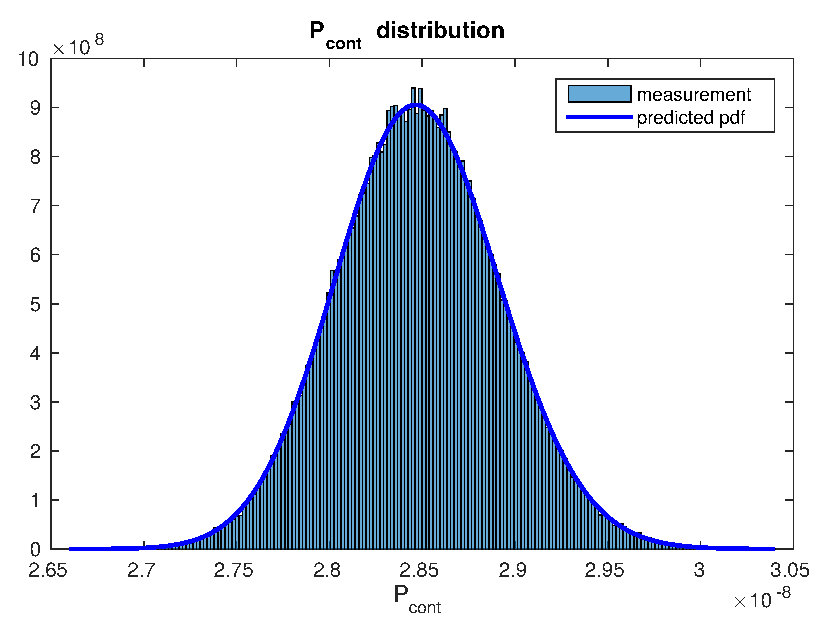
\includegraphics[width=0.5\textwidth]{figures/P_cont_40dBm_k100}%
	
	%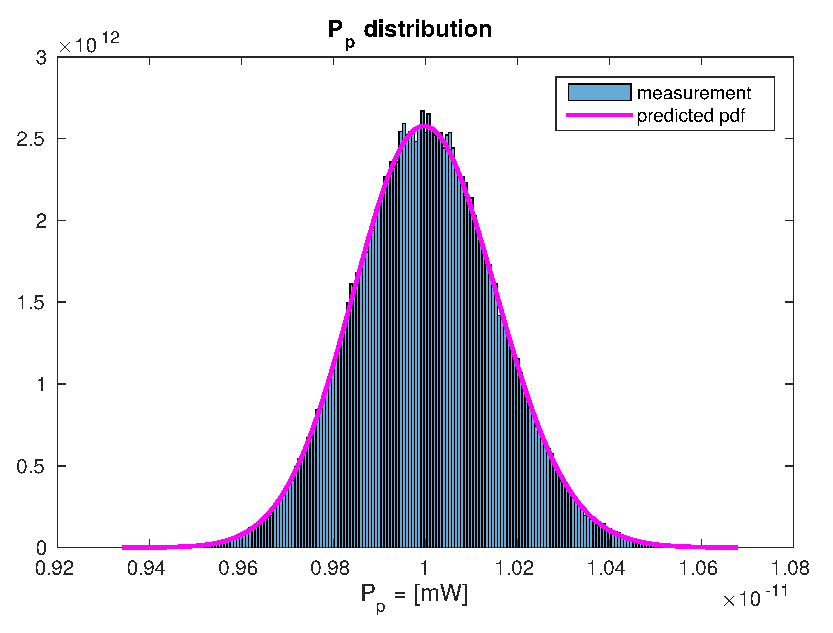
\includegraphics[width=0.5\textwidth]{figures/P_p_40dBm_k100}%
	%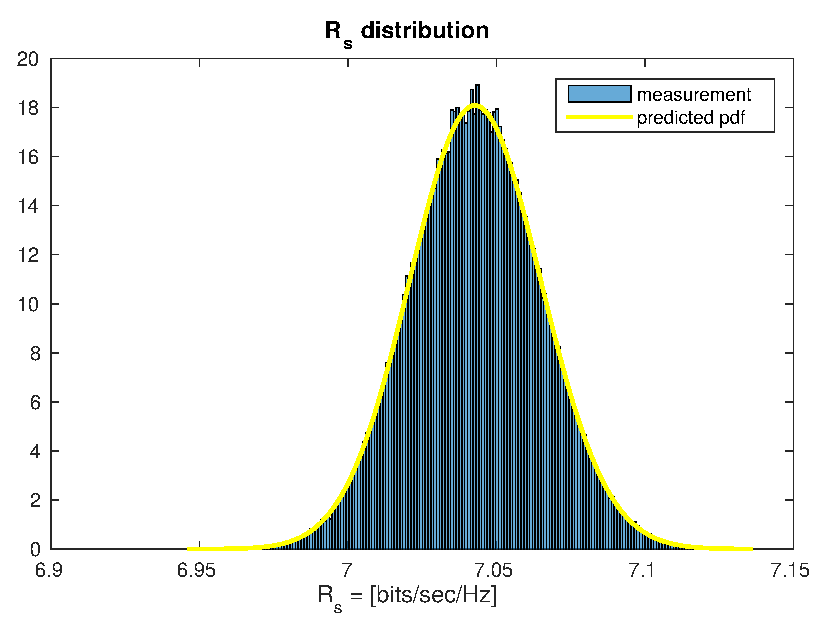
\includegraphics[width=0.5\textwidth]{figures/R_s_40dBm_k100}%
	\caption{Validating the theoretical expressions of the pdf and the experimental results with a certain choice of the system parameters depicted in Table \ref{param}.}
	\label{hrel_pdf}
	%\vspace{-10 pt}
\end{figure}

\begin{table}
%	%\vspace{-10 pt}
	%\setlength{\tabcolsep}{3pt} % spacing between columns
        \renewcommand{\arraystretch}{1.4}
	\centering
	\caption{$\epsilon$ for different values of $\snrrcvdu$}
	\label{nichtzentral}
	\begin{tabular}{c||c} 
		\bfseries $\snrrcvdu$/[dB] &  \bfseries $\epsilon$ \\ \hline \hline
		$4.08$ &  $0.0568$ \\
		$9.10$ &  $0.0601$ \\
		$14.11$ & $0.0522$ \\
		$19.12$ & $0.0437$ \\
		$24.09$ & $0.0506$ \\
		$29.09$ & $0.0634$ \\
		$34.03$ & $0.1179$ \\
		$39.38$ & $0.0800$ \\
		$45.08$ & $0.1695$ \\ \hline
		%$e_\textrm{rel}$ & $0.0568$ & $0.0601$ & $0.0522$ & $0.0437$ &	$0.0506$ & $0.0634$ & $0.1179$ & $0.0800$ & $0.1695$ \\ 
	\end{tabular}
%	\vspace{-10 pt} 
\end{table}


The experiments were repeated for different values of $\snrrcvdu$. It was observed that for a considerable range of $\snrrcvdu \in (4,30)$ $\SI{}{dB}$, the theoretical expressions depicted a significant accuracy to the experimental data, refer to Table \ref{nichtzentral}. The accuracy is quantified in terms of a relative error ($\epsilon$), defined as
\begin{equation}
\label{fr}
\epsilon = \frac{1}{|\mathcal X\sub{bins}|} \times \sum_{x \in \mathcal X\sub{bins}} \frac{\dprcvdstpr(x) - f\sub{hist}(x)}{f\sub{hist}(x)} \;  , 
\end{equation}
$|\mathcal X\sub{bins}|$ represents the cardinality of $\mathcal X\sub{bins}$, which excludes the bins with $f\sub{hist}(x) = 0$. The different values of $\snrrcvdu$ correspond to the different channel conditions. Hence, this observation concludes that the proposed framework is robust to the fluctuations in the channel gain. 

\subsection{Validation of Estimation-Throughput Tradeoff}
\index{Hardware validation!estimation-throughput tradeoff}
\begin{figure}
	%\vspace{-20 pt}
	\centering
	% This file is generated by the MATLAB m-file laprint.m. It can be included
% into LaTeX documents using the packages graphicx, color and psfrag.
% It is accompanied by a postscript file. A sample LaTeX file is:
%    \documentclass{article}\usepackage{graphicx,color,psfrag}
%    \begin{document}% This file is generated by the MATLAB m-file laprint.m. It can be included
% into LaTeX documents using the packages graphicx, color and psfrag.
% It is accompanied by a postscript file. A sample LaTeX file is:
%    \documentclass{article}\usepackage{graphicx,color,psfrag}
%    \begin{document}% This file is generated by the MATLAB m-file laprint.m. It can be included
% into LaTeX documents using the packages graphicx, color and psfrag.
% It is accompanied by a postscript file. A sample LaTeX file is:
%    \documentclass{article}\usepackage{graphicx,color,psfrag}
%    \begin{document}\input{ETT}\end{document}
% See http://www.mathworks.de/matlabcentral/fileexchange/loadFile.do?objectId=4638
% for recent versions of laprint.m.
%
% created by:           LaPrint version 3.16 (13.9.2004)
% created on:           23-Mar-2016 13:43:56
% eps bounding box:     16 cm x 12 cm
% comment:              
%
%\begin{psfrags}%
%\psfragscanon%
%
% text strings:
\psfrag{s06}[t][t]{\fontsize{8}{12}\fontseries{m}\mathversion{normal}\fontshape{n}\selectfont \color[rgb]{0,0,0}\setlength{\tabcolsep}{0pt}\begin{tabular}{c}$\test = [\SI{}{ms}]$\end{tabular}}%
\psfrag{s07}[b][b]{\fontsize{8}{12}\fontseries{m}\mathversion{normal}\fontshape{n}\selectfont \color[rgb]{0,0,0}\setlength{\tabcolsep}{0pt}\begin{tabular}{c}$\e{\ers}{\ers}  = [\SI{}{bits/s/Hz}]$\end{tabular}}%
\psfrag{s11}[][]{\fontsize{10}{15}\fontseries{m}\mathversion{normal}\fontshape{n}\selectfont \color[rgb]{0,0,0}\setlength{\tabcolsep}{0pt}\begin{tabular}{c} \end{tabular}}%
\psfrag{s12}[][]{\fontsize{10}{15}\fontseries{m}\mathversion{normal}\fontshape{n}\selectfont \color[rgb]{0,0,0}\setlength{\tabcolsep}{0pt}\begin{tabular}{c} \end{tabular}}%
\psfrag{s14}[t][t]{\fontsize{8}{12}\fontseries{m}\mathversion{normal}\fontshape{n}\selectfont \color[rgb]{0,0,0}\setlength{\tabcolsep}{0pt}\begin{tabular}{c}$\pco$\end{tabular}}%
\psfrag{s18}[l][l]{\fontsize{8}{12}\fontseries{m}\mathversion{normal}\fontshape{n}\selectfont \color[rgb]{0,0,0}Empirical}%
\psfrag{s19}[l][l]{\fontsize{8}{12}\fontseries{m}\mathversion{normal}\fontshape{n}\selectfont \color[rgb]{0,0,0}$\e{\ers}{\ers}$]}%
\psfrag{s20}[l][l]{\fontsize{8}{12}\fontseries{m}\mathversion{normal}\fontshape{n}\selectfont \color[rgb]{0,0,0}$\pco$}%
\psfrag{s21}[l][l]{\fontsize{8}{12}\fontseries{m}\mathversion{normal}\fontshape{n}\selectfont \color[rgb]{0,0,0}Empirical}%
%
% axes font properties:
\fontsize{8}{12}\fontseries{m}\mathversion{normal}%
\fontshape{n}\selectfont%
%
% xticklabels:
\psfrag{x01}[t][t]{0}%
\psfrag{x02}[t][t]{0.5}%
\psfrag{x03}[t][t]{1}%
\psfrag{x04}[t][t]{1.5}%
\psfrag{x05}[t][t]{2}%
\psfrag{x06}[t][t]{2.5}%
\psfrag{x07}[t][t]{0}%
\psfrag{x08}[t][t]{0.5}%
\psfrag{x09}[t][t]{1}%
\psfrag{x10}[t][t]{1.5}%
\psfrag{x11}[t][t]{2}%
\psfrag{x12}[t][t]{2.5}%
%
% yticklabels:
\psfrag{v01}[l][l]{0.50}%
\psfrag{v02}[l][l]{0.60}%
\psfrag{v03}[l][l]{0.70}%
\psfrag{v04}[l][l]{0.80}%
\psfrag{v05}[l][l]{0.90}%
\psfrag{v06}[l][l]{1.00}%
\psfrag{v07}[l][l]{}%
\psfrag{v08}[r][r]{6.89}%
\psfrag{v09}[r][r]{6.93}%
\psfrag{v10}[r][r]{6.96}%
\psfrag{v11}[r][r]{7.00}%
\psfrag{v12}[r][r]{7.04}%
\psfrag{v13}[r][r]{7.07}%
\psfrag{v14}[r][r]{}%
%
% Figure:
%\resizebox{8cm}{!}{\includegraphics{ETT.eps}}%
%\end{psfrags}%
%
% End ETT.tex
\end{document}
% See http://www.mathworks.de/matlabcentral/fileexchange/loadFile.do?objectId=4638
% for recent versions of laprint.m.
%
% created by:           LaPrint version 3.16 (13.9.2004)
% created on:           23-Mar-2016 13:43:56
% eps bounding box:     16 cm x 12 cm
% comment:              
%
%\begin{psfrags}%
%\psfragscanon%
%
% text strings:
\psfrag{s06}[t][t]{\fontsize{8}{12}\fontseries{m}\mathversion{normal}\fontshape{n}\selectfont \color[rgb]{0,0,0}\setlength{\tabcolsep}{0pt}\begin{tabular}{c}$\test = [\SI{}{ms}]$\end{tabular}}%
\psfrag{s07}[b][b]{\fontsize{8}{12}\fontseries{m}\mathversion{normal}\fontshape{n}\selectfont \color[rgb]{0,0,0}\setlength{\tabcolsep}{0pt}\begin{tabular}{c}$\e{\ers}{\ers}  = [\SI{}{bits/s/Hz}]$\end{tabular}}%
\psfrag{s11}[][]{\fontsize{10}{15}\fontseries{m}\mathversion{normal}\fontshape{n}\selectfont \color[rgb]{0,0,0}\setlength{\tabcolsep}{0pt}\begin{tabular}{c} \end{tabular}}%
\psfrag{s12}[][]{\fontsize{10}{15}\fontseries{m}\mathversion{normal}\fontshape{n}\selectfont \color[rgb]{0,0,0}\setlength{\tabcolsep}{0pt}\begin{tabular}{c} \end{tabular}}%
\psfrag{s14}[t][t]{\fontsize{8}{12}\fontseries{m}\mathversion{normal}\fontshape{n}\selectfont \color[rgb]{0,0,0}\setlength{\tabcolsep}{0pt}\begin{tabular}{c}$\pco$\end{tabular}}%
\psfrag{s18}[l][l]{\fontsize{8}{12}\fontseries{m}\mathversion{normal}\fontshape{n}\selectfont \color[rgb]{0,0,0}Empirical}%
\psfrag{s19}[l][l]{\fontsize{8}{12}\fontseries{m}\mathversion{normal}\fontshape{n}\selectfont \color[rgb]{0,0,0}$\e{\ers}{\ers}$]}%
\psfrag{s20}[l][l]{\fontsize{8}{12}\fontseries{m}\mathversion{normal}\fontshape{n}\selectfont \color[rgb]{0,0,0}$\pco$}%
\psfrag{s21}[l][l]{\fontsize{8}{12}\fontseries{m}\mathversion{normal}\fontshape{n}\selectfont \color[rgb]{0,0,0}Empirical}%
%
% axes font properties:
\fontsize{8}{12}\fontseries{m}\mathversion{normal}%
\fontshape{n}\selectfont%
%
% xticklabels:
\psfrag{x01}[t][t]{0}%
\psfrag{x02}[t][t]{0.5}%
\psfrag{x03}[t][t]{1}%
\psfrag{x04}[t][t]{1.5}%
\psfrag{x05}[t][t]{2}%
\psfrag{x06}[t][t]{2.5}%
\psfrag{x07}[t][t]{0}%
\psfrag{x08}[t][t]{0.5}%
\psfrag{x09}[t][t]{1}%
\psfrag{x10}[t][t]{1.5}%
\psfrag{x11}[t][t]{2}%
\psfrag{x12}[t][t]{2.5}%
%
% yticklabels:
\psfrag{v01}[l][l]{0.50}%
\psfrag{v02}[l][l]{0.60}%
\psfrag{v03}[l][l]{0.70}%
\psfrag{v04}[l][l]{0.80}%
\psfrag{v05}[l][l]{0.90}%
\psfrag{v06}[l][l]{1.00}%
\psfrag{v07}[l][l]{}%
\psfrag{v08}[r][r]{6.89}%
\psfrag{v09}[r][r]{6.93}%
\psfrag{v10}[r][r]{6.96}%
\psfrag{v11}[r][r]{7.00}%
\psfrag{v12}[r][r]{7.04}%
\psfrag{v13}[r][r]{7.07}%
\psfrag{v14}[r][r]{}%
%
% Figure:
%\resizebox{8cm}{!}{\includegraphics{ETT.eps}}%
%\end{psfrags}%
%
% End ETT.tex
\end{document}
% See http://www.mathworks.de/matlabcentral/fileexchange/loadFile.do?objectId=4638
% for recent versions of laprint.m.
%
% created by:           LaPrint version 3.16 (13.9.2004)
% created on:           23-Mar-2016 13:43:56
% eps bounding box:     16 cm x 12 cm
% comment:              
%
%\begin{psfrags}%
%\psfragscanon%
%
% text strings:
\psfrag{s06}[t][t]{\fontsize{8}{12}\fontseries{m}\mathversion{normal}\fontshape{n}\selectfont \color[rgb]{0,0,0}\setlength{\tabcolsep}{0pt}\begin{tabular}{c}$\test = [\SI{}{ms}]$\end{tabular}}%
\psfrag{s07}[b][b]{\fontsize{8}{12}\fontseries{m}\mathversion{normal}\fontshape{n}\selectfont \color[rgb]{0,0,0}\setlength{\tabcolsep}{0pt}\begin{tabular}{c}$\e{\ers}{\ers}  = [\SI{}{bits/s/Hz}]$\end{tabular}}%
\psfrag{s11}[][]{\fontsize{10}{15}\fontseries{m}\mathversion{normal}\fontshape{n}\selectfont \color[rgb]{0,0,0}\setlength{\tabcolsep}{0pt}\begin{tabular}{c} \end{tabular}}%
\psfrag{s12}[][]{\fontsize{10}{15}\fontseries{m}\mathversion{normal}\fontshape{n}\selectfont \color[rgb]{0,0,0}\setlength{\tabcolsep}{0pt}\begin{tabular}{c} \end{tabular}}%
\psfrag{s14}[t][t]{\fontsize{8}{12}\fontseries{m}\mathversion{normal}\fontshape{n}\selectfont \color[rgb]{0,0,0}\setlength{\tabcolsep}{0pt}\begin{tabular}{c}$\pco$\end{tabular}}%
\psfrag{s18}[l][l]{\fontsize{8}{12}\fontseries{m}\mathversion{normal}\fontshape{n}\selectfont \color[rgb]{0,0,0}Empirical}%
\psfrag{s19}[l][l]{\fontsize{8}{12}\fontseries{m}\mathversion{normal}\fontshape{n}\selectfont \color[rgb]{0,0,0}$\e{\ers}{\ers}$]}%
\psfrag{s20}[l][l]{\fontsize{8}{12}\fontseries{m}\mathversion{normal}\fontshape{n}\selectfont \color[rgb]{0,0,0}$\pco$}%
\psfrag{s21}[l][l]{\fontsize{8}{12}\fontseries{m}\mathversion{normal}\fontshape{n}\selectfont \color[rgb]{0,0,0}Empirical}%
%
% axes font properties:
\fontsize{8}{12}\fontseries{m}\mathversion{normal}%
\fontshape{n}\selectfont%
%
% xticklabels:
\psfrag{x01}[t][t]{0}%
\psfrag{x02}[t][t]{0.5}%
\psfrag{x03}[t][t]{1}%
\psfrag{x04}[t][t]{1.5}%
\psfrag{x05}[t][t]{2}%
\psfrag{x06}[t][t]{2.5}%
\psfrag{x07}[t][t]{0}%
\psfrag{x08}[t][t]{0.5}%
\psfrag{x09}[t][t]{1}%
\psfrag{x10}[t][t]{1.5}%
\psfrag{x11}[t][t]{2}%
\psfrag{x12}[t][t]{2.5}%
%
% yticklabels:
\psfrag{v01}[l][l]{0.50}%
\psfrag{v02}[l][l]{0.60}%
\psfrag{v03}[l][l]{0.70}%
\psfrag{v04}[l][l]{0.80}%
\psfrag{v05}[l][l]{0.90}%
\psfrag{v06}[l][l]{1.00}%
\psfrag{v07}[l][l]{}%
\psfrag{v08}[r][r]{6.89}%
\psfrag{v09}[r][r]{6.93}%
\psfrag{v10}[r][r]{6.96}%
\psfrag{v11}[r][r]{7.00}%
\psfrag{v12}[r][r]{7.04}%
\psfrag{v13}[r][r]{7.07}%
\psfrag{v14}[r][r]{}%
%
% Figure:
%\resizebox{8cm}{!}{\includegraphics{ETT.eps}}%
%\end{psfrags}%
%
% End ETT.tex

	\begin{tikzpicture}[scale=1]
        \node[anchor=south west,inner sep=0] (image) at (0,0)
        {
		\includegraphics[width=\figscale]{figures/ETT}
	};
        \begin{scope}[x={(image.south east)},y={(image.north west)}]
        \node[draw, fill=gray!10,font=\scriptsize] (text1) at (0.98,0.872) {$\pcod$};
	\draw[black, ->] (text1.west) -- (0.913,0.872);
        
	\node[draw, fill=gray!10,font=\scriptsize] (text2) at (0.3275,0.01) {$\ttest$};
	\draw[black, ->] (text2.north) -- (0.3275,0.086);
        
	\node[draw, fill=gray!10,font=\scriptsize] (text3) at (-0.06,0.9) {$\maxi\e{\ers}{\ers}$};
	\draw[black, ->] (text3.south) -- (0.084,0.7);

                %\draw[help lines,xstep=.1,ystep=.1] (0,0) grid (1,1);
                %\foreach \x in {0,1,...,9} { \node [anchor=north] at (\x/10,0) {0.\x}; }
                %\foreach \y in {0,1,...,9} { \node [anchor=east] at (0,\y/10) {0.\y}; }
                \end{scope}
        \end{tikzpicture}
	\caption{Validating the estimation-throughput tradeoff for the choice of parameters depicted in Table \ref{param}. The figure illustrates the suitable estimation time $\ttest$ at which the confidence probability is satisfied, see the projection of $\square$ on the curve $\pco$, at the same time achieves the maximum expected secondary throughput, see the projection of $\Box$ on the curve $\e{\ers}{\ers}$.} 

	\label{RspocstricheA}
\end{figure}

Following the validation of the pdfs that captures the variations in the system parameters, it is interesting to validate the performance of the CR system in terms of the estimation-throughput tradeoff, characterized in (\ref{eq_HVD:sys}). Thus, the feasibility of the optimization problem that respects the interference constraint on $\pco$ is validated. As discussed previously, a large $\test$ improves the performance of the primary system by reducing the variations in $\eprcvdpr$, depicted by observing an increase in $\pco$, cf. \figurename~\ref{RspocstricheA}. Conversely, from the perspective of the secondary system, the increase in $\test$ reduces the expected secondary throughput. 

These variations of the expected throughput and the confidence probability versus the estimation time are presented in \figurename~\ref{RspocstricheA}, which illustrates a joint validation of the performance parameters ($\e{\ers}{\ers}$ and $\pco$) of the underlay CR system. Again, the validation is achieved by comparing the measurements of the performance parameters with their analytical expressions for different $\test$. In contrast to the analytical framework, presented in Section \ref{model}, the empirical values of $\pco$ are determined by computing a numerical integration in the region within the confidence interval $(1  \pm \acc)  \theta_\textrm{I}$, cf. \figurename~\ref{hrel_pdf}. 

After performing the validation, following conclusions can be outlined: 
\begin{itemize}
\item The accuracy of the derived expressions and the feasibility of the received power-based estimation (proposed in this thesis) have been justified by means of a hardware realization.
\item Furthermore, in accordance to the validation process, the applicability of the simplifications and solutions, proposed in Section \ref{ssec:simp1}, has been accounted.    
\end{itemize}
This signifies that the proposed framework is capable of illustrating the underlay principle by means of a demonstrator.
\index{Hardware validation|)}

\section{Hardware Demonstration}
\index{Demonstrator|(}
\label{sec:demo}
Although the validation is an important part of the system design, it is restricted to offline verification of the proposed approach. From a deployment perspective, it is interesting to demonstrate the online operation of the underlay paradigm on the hardware. This section provides insights on the involved challenges while deploying the proposed approach in the form of a demonstrator. In the thesis, the operation of CR systems at a suitable estimation time that is associated with the maximum secondary throughput has been analyzed, which represents the optimum performance of a CR system. However, in practice, it is difficult to determine the value of this parameter while the system is operating -- \textit{on the fly}. In this regard, the subsequent section discusses this challenging task and proposes a heuristic approach of determining the estimation time. 

\subsection{Determining Estimation Time}
\label{esttime}
The analytical expression (\ref{eq_HVD:sys}) and \figurename~\ref{RspocstricheA} illustrate a dependency of the performance parameters ($\pco$ and $\e{\ers}{\ers}$) on the estimation time $\test$. This dependency, depicted as the estimation-throughput tradeoff, is utilized to determine the suitable estimation time $\ttest$ that achieves the maximum secondary throughput. However, $\ttest$ can be determined for a certain value of the $\snrrcvdu$, which represents a certain channel gain. In practice, the mobility of the ST or the PR, or the surroundings objects cause variations in the channel gain, which consequently induce variations in the received $\snrrcvdu$. Under this situation, it is challenging to select $\ttest$ such that the system adheres to the confidence probability constraint and still achieves the maximum secondary throughput for a corresponding range of $\snrrcvdu$. 

To approach this issue, the variation of $\ttest$ for a certain range of $\snrrcvdu$ and different values of the confidence probability constraint $\pcod \in \{0.90, 0.95, 0.99\}$ is investigated\footnote{Such investigations can be performed during the validation process, which is normally included at the system design.}, cf. \figurename~\ref{fig_HVD:Tausnr}. %a new parameter called the estimation time ($\testo$) is introduced. It is $\test$ that maximizes the secondary throughput according to (\ref{eq_HVD:}) in \cite{Kaushik15} for a certain value of $\snrrcvd$, $\mu$ and a target value of $P_\textrm{c}$ defined as $\bar{P_\textrm{c}}$. In Fig. \ref{RspocstricheA}, this optimization process is indicated graphically by the dotted lines, where, from a fixed $\bar{P_\textrm{c}} = 0.95$, we acquire $\tau_\textrm{opt} \approx \SI{0.75}{ms}$, which corresponds to $\mathbb{E}\left[R_\textrm{s}\right] \approx \SI{7.02}{bits/s/Hz}$.
%However, this analysis is carried out for a fixed value of $\snrrcvd$. Under real conditions, due to channel fading, $\snrrcvd$ is not known. In this sense, it is not possible to determine $\tau_\textrm{opt}$. To resolve this issue, we propose a procedure, whereby we analyze the variations of $\tau_\textrm{opt}$ for different values of $\snrrcvd$, refer to Fig. \ref{Tausnr}, and select $\tau_\textrm{opt}$'s maximum value. 
Thus, the maximum value of the suitable estimation time for a certain range of $\snrrcvdu$ and $\pcod$ is selected as the estimation time for the demonstrator, given by \begin{equation}
\ttesto = \maxi\{ \ttest | \snrrcvdu \in (-10,20)\;\SI{}{dB}; \;\pco = \pcod \}.\end{equation} Since the $\ttesto$ is not optimal for all $\snrrcvdu$, it is different from $\ttest$. Hence, a different notation is assigned for its representation. By doing this, it is assured that the confidence probability constraint is satisfied for different realizations of the channel gain, which reside within the interval $\snrrcvdu \in (-10,20)$ $\SI{}{dB}$. 
%In addition, we consider different values of $\bar{P_\textrm{c}}$. 
%\begin{figure}
%	%\vspace{-10 pt}
%	\centering
%	% This file is generated by the MATLAB m-file laprint.m. It can be included
% into LaTeX documents using the packages graphicx, color and psfrag.
% It is accompanied by a postscript file. A sample LaTeX file is:
%    \documentclass{article}\usepackage{graphicx,color,psfrag}
%    \begin{document}% This file is generated by the MATLAB m-file laprint.m. It can be included
% into LaTeX documents using the packages graphicx, color and psfrag.
% It is accompanied by a postscript file. A sample LaTeX file is:
%    \documentclass{article}\usepackage{graphicx,color,psfrag}
%    \begin{document}% This file is generated by the MATLAB m-file laprint.m. It can be included
% into LaTeX documents using the packages graphicx, color and psfrag.
% It is accompanied by a postscript file. A sample LaTeX file is:
%    \documentclass{article}\usepackage{graphicx,color,psfrag}
%    \begin{document}\input{Rs_SNR}\end{document}
% See http://www.mathworks.de/matlabcentral/fileexchange/loadFile.do?objectId=4638
% for recent versions of laprint.m.
%
% created by:           LaPrint version 3.16 (13.9.2004)
% created on:           01-Apr-2016 10:23:46
% eps bounding box:     16 cm x 12 cm
% comment:              
%
%\begin{psfrags}%
%\psfragscanon%
%
% text strings:
\psfrag{s05}[t][t]{\fontsize{8}{12}\fontseries{m}\mathversion{normal}\fontshape{n}\selectfont \color[rgb]{0,0,0}\setlength{\tabcolsep}{0pt}\begin{tabular}{c}$\snrrcvd = [\SI{}{dB}]$\end{tabular}}%
\psfrag{s06}[b][b]{\fontsize{8}{12}\fontseries{m}\mathversion{normal}\fontshape{n}\selectfont \color[rgb]{0,0,0}\setlength{\tabcolsep}{0pt}\begin{tabular}{c}$\e{ers}{\ers(\ttest)} = [\SI{}{bits/s/Hz}]$\end{tabular}}%
\psfrag{s10}[][]{\fontsize{10}{15}\fontseries{m}\mathversion{normal}\fontshape{n}\selectfont \color[rgb]{0,0,0}\setlength{\tabcolsep}{0pt}\begin{tabular}{c} \end{tabular}}%
\psfrag{s11}[][]{\fontsize{10}{15}\fontseries{m}\mathversion{normal}\fontshape{n}\selectfont \color[rgb]{0,0,0}\setlength{\tabcolsep}{0pt}\begin{tabular}{c} \end{tabular}}%
\psfrag{s12}[l][l]{\fontsize{8}{12}\fontseries{m}\mathversion{normal}\fontshape{n}\selectfont \color[rgb]{0,0,0}$\pcod = 0.99$}%
\psfrag{s13}[l][l]{\fontsize{8}{12}\fontseries{m}\mathversion{normal}\fontshape{n}\selectfont \color[rgb]{0,0,0}$\pcod = 0.90$}%
\psfrag{s14}[l][l]{\fontsize{8}{12}\fontseries{m}\mathversion{normal}\fontshape{n}\selectfont \color[rgb]{0,0,0}$\pcod = 0.95$}%
\psfrag{s15}[l][l]{\fontsize{8}{12}\fontseries{m}\mathversion{normal}\fontshape{n}\selectfont \color[rgb]{0,0,0}$\pcod = 0.99$}%
%
% axes font properties:
\fontsize{8}{12}\fontseries{m}\mathversion{normal}%
\fontshape{n}\selectfont%
%
% xticklabels:
\psfrag{x01}[t][t]{-10}%
\psfrag{x02}[t][t]{-5}%
\psfrag{x03}[t][t]{0}%
\psfrag{x04}[t][t]{5}%
\psfrag{x05}[t][t]{10}%
\psfrag{x06}[t][t]{15}%
%
% yticklabels:
\psfrag{v01}[r][r]{6}%
\psfrag{v02}[r][r]{6.5}%
\psfrag{v03}[r][r]{7}%
\psfrag{v04}[r][r]{7.5}%
\psfrag{v05}[r][r]{8}%
\psfrag{v06}[r][r]{8.5}%
\psfrag{v07}[r][r]{9}%
\psfrag{v08}[r][r]{9.5}%
\psfrag{v09}[r][r]{10}%
\psfrag{v10}[r][r]{10.5}%
\psfrag{v11}[r][r]{11}%
%
% Figure:
%\resizebox{8cm}{!}{\includegraphics{Rs_SNR.eps}}%
%\end{psfrags}%
%
% End Rs_SNR.tex
\end{document}
% See http://www.mathworks.de/matlabcentral/fileexchange/loadFile.do?objectId=4638
% for recent versions of laprint.m.
%
% created by:           LaPrint version 3.16 (13.9.2004)
% created on:           01-Apr-2016 10:23:46
% eps bounding box:     16 cm x 12 cm
% comment:              
%
%\begin{psfrags}%
%\psfragscanon%
%
% text strings:
\psfrag{s05}[t][t]{\fontsize{8}{12}\fontseries{m}\mathversion{normal}\fontshape{n}\selectfont \color[rgb]{0,0,0}\setlength{\tabcolsep}{0pt}\begin{tabular}{c}$\snrrcvd = [\SI{}{dB}]$\end{tabular}}%
\psfrag{s06}[b][b]{\fontsize{8}{12}\fontseries{m}\mathversion{normal}\fontshape{n}\selectfont \color[rgb]{0,0,0}\setlength{\tabcolsep}{0pt}\begin{tabular}{c}$\e{ers}{\ers(\ttest)} = [\SI{}{bits/s/Hz}]$\end{tabular}}%
\psfrag{s10}[][]{\fontsize{10}{15}\fontseries{m}\mathversion{normal}\fontshape{n}\selectfont \color[rgb]{0,0,0}\setlength{\tabcolsep}{0pt}\begin{tabular}{c} \end{tabular}}%
\psfrag{s11}[][]{\fontsize{10}{15}\fontseries{m}\mathversion{normal}\fontshape{n}\selectfont \color[rgb]{0,0,0}\setlength{\tabcolsep}{0pt}\begin{tabular}{c} \end{tabular}}%
\psfrag{s12}[l][l]{\fontsize{8}{12}\fontseries{m}\mathversion{normal}\fontshape{n}\selectfont \color[rgb]{0,0,0}$\pcod = 0.99$}%
\psfrag{s13}[l][l]{\fontsize{8}{12}\fontseries{m}\mathversion{normal}\fontshape{n}\selectfont \color[rgb]{0,0,0}$\pcod = 0.90$}%
\psfrag{s14}[l][l]{\fontsize{8}{12}\fontseries{m}\mathversion{normal}\fontshape{n}\selectfont \color[rgb]{0,0,0}$\pcod = 0.95$}%
\psfrag{s15}[l][l]{\fontsize{8}{12}\fontseries{m}\mathversion{normal}\fontshape{n}\selectfont \color[rgb]{0,0,0}$\pcod = 0.99$}%
%
% axes font properties:
\fontsize{8}{12}\fontseries{m}\mathversion{normal}%
\fontshape{n}\selectfont%
%
% xticklabels:
\psfrag{x01}[t][t]{-10}%
\psfrag{x02}[t][t]{-5}%
\psfrag{x03}[t][t]{0}%
\psfrag{x04}[t][t]{5}%
\psfrag{x05}[t][t]{10}%
\psfrag{x06}[t][t]{15}%
%
% yticklabels:
\psfrag{v01}[r][r]{6}%
\psfrag{v02}[r][r]{6.5}%
\psfrag{v03}[r][r]{7}%
\psfrag{v04}[r][r]{7.5}%
\psfrag{v05}[r][r]{8}%
\psfrag{v06}[r][r]{8.5}%
\psfrag{v07}[r][r]{9}%
\psfrag{v08}[r][r]{9.5}%
\psfrag{v09}[r][r]{10}%
\psfrag{v10}[r][r]{10.5}%
\psfrag{v11}[r][r]{11}%
%
% Figure:
%\resizebox{8cm}{!}{\includegraphics{Rs_SNR.eps}}%
%\end{psfrags}%
%
% End Rs_SNR.tex
\end{document}
% See http://www.mathworks.de/matlabcentral/fileexchange/loadFile.do?objectId=4638
% for recent versions of laprint.m.
%
% created by:           LaPrint version 3.16 (13.9.2004)
% created on:           01-Apr-2016 10:23:46
% eps bounding box:     16 cm x 12 cm
% comment:              
%
%\begin{psfrags}%
%\psfragscanon%
%
% text strings:
\psfrag{s05}[t][t]{\fontsize{8}{12}\fontseries{m}\mathversion{normal}\fontshape{n}\selectfont \color[rgb]{0,0,0}\setlength{\tabcolsep}{0pt}\begin{tabular}{c}$\snrrcvd = [\SI{}{dB}]$\end{tabular}}%
\psfrag{s06}[b][b]{\fontsize{8}{12}\fontseries{m}\mathversion{normal}\fontshape{n}\selectfont \color[rgb]{0,0,0}\setlength{\tabcolsep}{0pt}\begin{tabular}{c}$\e{ers}{\ers(\ttest)} = [\SI{}{bits/s/Hz}]$\end{tabular}}%
\psfrag{s10}[][]{\fontsize{10}{15}\fontseries{m}\mathversion{normal}\fontshape{n}\selectfont \color[rgb]{0,0,0}\setlength{\tabcolsep}{0pt}\begin{tabular}{c} \end{tabular}}%
\psfrag{s11}[][]{\fontsize{10}{15}\fontseries{m}\mathversion{normal}\fontshape{n}\selectfont \color[rgb]{0,0,0}\setlength{\tabcolsep}{0pt}\begin{tabular}{c} \end{tabular}}%
\psfrag{s12}[l][l]{\fontsize{8}{12}\fontseries{m}\mathversion{normal}\fontshape{n}\selectfont \color[rgb]{0,0,0}$\pcod = 0.99$}%
\psfrag{s13}[l][l]{\fontsize{8}{12}\fontseries{m}\mathversion{normal}\fontshape{n}\selectfont \color[rgb]{0,0,0}$\pcod = 0.90$}%
\psfrag{s14}[l][l]{\fontsize{8}{12}\fontseries{m}\mathversion{normal}\fontshape{n}\selectfont \color[rgb]{0,0,0}$\pcod = 0.95$}%
\psfrag{s15}[l][l]{\fontsize{8}{12}\fontseries{m}\mathversion{normal}\fontshape{n}\selectfont \color[rgb]{0,0,0}$\pcod = 0.99$}%
%
% axes font properties:
\fontsize{8}{12}\fontseries{m}\mathversion{normal}%
\fontshape{n}\selectfont%
%
% xticklabels:
\psfrag{x01}[t][t]{-10}%
\psfrag{x02}[t][t]{-5}%
\psfrag{x03}[t][t]{0}%
\psfrag{x04}[t][t]{5}%
\psfrag{x05}[t][t]{10}%
\psfrag{x06}[t][t]{15}%
%
% yticklabels:
\psfrag{v01}[r][r]{6}%
\psfrag{v02}[r][r]{6.5}%
\psfrag{v03}[r][r]{7}%
\psfrag{v04}[r][r]{7.5}%
\psfrag{v05}[r][r]{8}%
\psfrag{v06}[r][r]{8.5}%
\psfrag{v07}[r][r]{9}%
\psfrag{v08}[r][r]{9.5}%
\psfrag{v09}[r][r]{10}%
\psfrag{v10}[r][r]{10.5}%
\psfrag{v11}[r][r]{11}%
%
% Figure:
%\resizebox{8cm}{!}{\includegraphics{Rs_SNR.eps}}%
%\end{psfrags}%
%
% End Rs_SNR.tex

%	\includegraphics[width=\figscale]{figures/Rs_SNR}
%	\caption{$\tau_\textrm{opt}$ over $\snrrcvd$, $\theta_\textrm{I}$ = \SI{-110}{dBm}, $\mu$ = 0.05}
%	\label{fig_HVD:Tausnr}
%	%\vspace{-10 pt}
%\end{figure}
\begin{figure}
	%\vspace{-10 pt}
	\centering
	% This file is generated by the MATLAB m-file laprint.m. It can be included
% into LaTeX documents using the packages graphicx, color and psfrag.
% It is accompanied by a postscript file. A sample LaTeX file is:
%    \documentclass{article}\usepackage{graphicx,color,psfrag}
%    \begin{document}% This file is generated by the MATLAB m-file laprint.m. It can be included
% into LaTeX documents using the packages graphicx, color and psfrag.
% It is accompanied by a postscript file. A sample LaTeX file is:
%    \documentclass{article}\usepackage{graphicx,color,psfrag}
%    \begin{document}% This file is generated by the MATLAB m-file laprint.m. It can be included
% into LaTeX documents using the packages graphicx, color and psfrag.
% It is accompanied by a postscript file. A sample LaTeX file is:
%    \documentclass{article}\usepackage{graphicx,color,psfrag}
%    \begin{document}\input{test_SNR}\end{document}
% See http://www.mathworks.de/matlabcentral/fileexchange/loadFile.do?objectId=4638
% for recent versions of laprint.m.
%
% created by:           LaPrint version 3.16 (13.9.2004)
% created on:           01-Apr-2016 10:23:47
% eps bounding box:     16 cm x 12 cm
% comment:              
%
%\begin{psfrags}%
%\psfragscanon%
%
% text strings:
\psfrag{s05}[t][t]{\fontsize{8}{12}\fontseries{m}\mathversion{normal}\fontshape{n}\selectfont \color[rgb]{0,0,0}\setlength{\tabcolsep}{0pt}\begin{tabular}{c}$\snrrcvd = [\SI{}{dB}]$\end{tabular}}%
\psfrag{s06}[b][b]{\fontsize{8}{12}\fontseries{m}\mathversion{normal}\fontshape{n}\selectfont \color[rgb]{0,0,0}\setlength{\tabcolsep}{0pt}\begin{tabular}{c}$\ttest = [\SI{}{ms}]$\end{tabular}}%
\psfrag{s10}[][]{\fontsize{10}{15}\fontseries{m}\mathversion{normal}\fontshape{n}\selectfont \color[rgb]{0,0,0}\setlength{\tabcolsep}{0pt}\begin{tabular}{c} \end{tabular}}%
\psfrag{s11}[][]{\fontsize{10}{15}\fontseries{m}\mathversion{normal}\fontshape{n}\selectfont \color[rgb]{0,0,0}\setlength{\tabcolsep}{0pt}\begin{tabular}{c} \end{tabular}}%
\psfrag{s12}[l][l]{\fontsize{8}{12}\fontseries{m}\mathversion{normal}\fontshape{n}\selectfont \color[rgb]{0,0,0}$\pcod = 0.99$}%
\psfrag{s13}[l][l]{\fontsize{8}{12}\fontseries{m}\mathversion{normal}\fontshape{n}\selectfont \color[rgb]{0,0,0}$\pcod = 0.90$}%
\psfrag{s14}[l][l]{\fontsize{8}{12}\fontseries{m}\mathversion{normal}\fontshape{n}\selectfont \color[rgb]{0,0,0}$\pcod = 0.95$}%
\psfrag{s15}[l][l]{\fontsize{8}{12}\fontseries{m}\mathversion{normal}\fontshape{n}\selectfont \color[rgb]{0,0,0}$\pcod = 0.99$}%
%
% axes font properties:
\fontsize{8}{12}\fontseries{m}\mathversion{normal}%
\fontshape{n}\selectfont%
%
% xticklabels:
\psfrag{x01}[t][t]{-10}%
\psfrag{x02}[t][t]{-5}%
\psfrag{x03}[t][t]{0}%
\psfrag{x04}[t][t]{5}%
\psfrag{x05}[t][t]{10}%
\psfrag{x06}[t][t]{15}%
%
% yticklabels:
\psfrag{v01}[r][r]{0}%
\psfrag{v02}[r][r]{5}%
\psfrag{v03}[r][r]{10}%
\psfrag{v04}[r][r]{15}%
\psfrag{v05}[r][r]{20}%
\psfrag{v06}[r][r]{25}%
\psfrag{v07}[r][r]{30}%
\psfrag{v08}[r][r]{35}%
\psfrag{v09}[r][r]{40}%
\psfrag{v10}[r][r]{45}%
%
% Figure:
%\resizebox{8cm}{!}{\includegraphics{test_SNR.eps}}%
%\end{psfrags}%
%
% End test_SNR.tex
\end{document}
% See http://www.mathworks.de/matlabcentral/fileexchange/loadFile.do?objectId=4638
% for recent versions of laprint.m.
%
% created by:           LaPrint version 3.16 (13.9.2004)
% created on:           01-Apr-2016 10:23:47
% eps bounding box:     16 cm x 12 cm
% comment:              
%
%\begin{psfrags}%
%\psfragscanon%
%
% text strings:
\psfrag{s05}[t][t]{\fontsize{8}{12}\fontseries{m}\mathversion{normal}\fontshape{n}\selectfont \color[rgb]{0,0,0}\setlength{\tabcolsep}{0pt}\begin{tabular}{c}$\snrrcvd = [\SI{}{dB}]$\end{tabular}}%
\psfrag{s06}[b][b]{\fontsize{8}{12}\fontseries{m}\mathversion{normal}\fontshape{n}\selectfont \color[rgb]{0,0,0}\setlength{\tabcolsep}{0pt}\begin{tabular}{c}$\ttest = [\SI{}{ms}]$\end{tabular}}%
\psfrag{s10}[][]{\fontsize{10}{15}\fontseries{m}\mathversion{normal}\fontshape{n}\selectfont \color[rgb]{0,0,0}\setlength{\tabcolsep}{0pt}\begin{tabular}{c} \end{tabular}}%
\psfrag{s11}[][]{\fontsize{10}{15}\fontseries{m}\mathversion{normal}\fontshape{n}\selectfont \color[rgb]{0,0,0}\setlength{\tabcolsep}{0pt}\begin{tabular}{c} \end{tabular}}%
\psfrag{s12}[l][l]{\fontsize{8}{12}\fontseries{m}\mathversion{normal}\fontshape{n}\selectfont \color[rgb]{0,0,0}$\pcod = 0.99$}%
\psfrag{s13}[l][l]{\fontsize{8}{12}\fontseries{m}\mathversion{normal}\fontshape{n}\selectfont \color[rgb]{0,0,0}$\pcod = 0.90$}%
\psfrag{s14}[l][l]{\fontsize{8}{12}\fontseries{m}\mathversion{normal}\fontshape{n}\selectfont \color[rgb]{0,0,0}$\pcod = 0.95$}%
\psfrag{s15}[l][l]{\fontsize{8}{12}\fontseries{m}\mathversion{normal}\fontshape{n}\selectfont \color[rgb]{0,0,0}$\pcod = 0.99$}%
%
% axes font properties:
\fontsize{8}{12}\fontseries{m}\mathversion{normal}%
\fontshape{n}\selectfont%
%
% xticklabels:
\psfrag{x01}[t][t]{-10}%
\psfrag{x02}[t][t]{-5}%
\psfrag{x03}[t][t]{0}%
\psfrag{x04}[t][t]{5}%
\psfrag{x05}[t][t]{10}%
\psfrag{x06}[t][t]{15}%
%
% yticklabels:
\psfrag{v01}[r][r]{0}%
\psfrag{v02}[r][r]{5}%
\psfrag{v03}[r][r]{10}%
\psfrag{v04}[r][r]{15}%
\psfrag{v05}[r][r]{20}%
\psfrag{v06}[r][r]{25}%
\psfrag{v07}[r][r]{30}%
\psfrag{v08}[r][r]{35}%
\psfrag{v09}[r][r]{40}%
\psfrag{v10}[r][r]{45}%
%
% Figure:
%\resizebox{8cm}{!}{\includegraphics{test_SNR.eps}}%
%\end{psfrags}%
%
% End test_SNR.tex
\end{document}
% See http://www.mathworks.de/matlabcentral/fileexchange/loadFile.do?objectId=4638
% for recent versions of laprint.m.
%
% created by:           LaPrint version 3.16 (13.9.2004)
% created on:           01-Apr-2016 10:23:47
% eps bounding box:     16 cm x 12 cm
% comment:              
%
%\begin{psfrags}%
%\psfragscanon%
%
% text strings:
\psfrag{s05}[t][t]{\fontsize{8}{12}\fontseries{m}\mathversion{normal}\fontshape{n}\selectfont \color[rgb]{0,0,0}\setlength{\tabcolsep}{0pt}\begin{tabular}{c}$\snrrcvd = [\SI{}{dB}]$\end{tabular}}%
\psfrag{s06}[b][b]{\fontsize{8}{12}\fontseries{m}\mathversion{normal}\fontshape{n}\selectfont \color[rgb]{0,0,0}\setlength{\tabcolsep}{0pt}\begin{tabular}{c}$\ttest = [\SI{}{ms}]$\end{tabular}}%
\psfrag{s10}[][]{\fontsize{10}{15}\fontseries{m}\mathversion{normal}\fontshape{n}\selectfont \color[rgb]{0,0,0}\setlength{\tabcolsep}{0pt}\begin{tabular}{c} \end{tabular}}%
\psfrag{s11}[][]{\fontsize{10}{15}\fontseries{m}\mathversion{normal}\fontshape{n}\selectfont \color[rgb]{0,0,0}\setlength{\tabcolsep}{0pt}\begin{tabular}{c} \end{tabular}}%
\psfrag{s12}[l][l]{\fontsize{8}{12}\fontseries{m}\mathversion{normal}\fontshape{n}\selectfont \color[rgb]{0,0,0}$\pcod = 0.99$}%
\psfrag{s13}[l][l]{\fontsize{8}{12}\fontseries{m}\mathversion{normal}\fontshape{n}\selectfont \color[rgb]{0,0,0}$\pcod = 0.90$}%
\psfrag{s14}[l][l]{\fontsize{8}{12}\fontseries{m}\mathversion{normal}\fontshape{n}\selectfont \color[rgb]{0,0,0}$\pcod = 0.95$}%
\psfrag{s15}[l][l]{\fontsize{8}{12}\fontseries{m}\mathversion{normal}\fontshape{n}\selectfont \color[rgb]{0,0,0}$\pcod = 0.99$}%
%
% axes font properties:
\fontsize{8}{12}\fontseries{m}\mathversion{normal}%
\fontshape{n}\selectfont%
%
% xticklabels:
\psfrag{x01}[t][t]{-10}%
\psfrag{x02}[t][t]{-5}%
\psfrag{x03}[t][t]{0}%
\psfrag{x04}[t][t]{5}%
\psfrag{x05}[t][t]{10}%
\psfrag{x06}[t][t]{15}%
%
% yticklabels:
\psfrag{v01}[r][r]{0}%
\psfrag{v02}[r][r]{5}%
\psfrag{v03}[r][r]{10}%
\psfrag{v04}[r][r]{15}%
\psfrag{v05}[r][r]{20}%
\psfrag{v06}[r][r]{25}%
\psfrag{v07}[r][r]{30}%
\psfrag{v08}[r][r]{35}%
\psfrag{v09}[r][r]{40}%
\psfrag{v10}[r][r]{45}%
%
% Figure:
%\resizebox{8cm}{!}{\includegraphics{test_SNR.eps}}%
%\end{psfrags}%
%
% End test_SNR.tex

	\includegraphics[width=\figscale]{figures/test_SNR}
	\caption{The variation of the suitable estimation time ($\ttest$) versus the received signal to noise ratio at the ST ($\snrrcvdu$) for different values of confidence probability constraint $\pcod \in \{0.90,0.95,0.99 \}$.}
	\label{fig_HVD:Tausnr}
	%\vspace{-10 pt}
\end{figure}

Besides, from \figurename~\ref{fig_HVD:Tausnr}, it is further observed that $\ttest$ decreases monotonically with $\snrrcvdu$. Below a certain $\snrrcvdu$, the descent, is slow in beginning and then increases tremendously. %\footnote{For varying $\theta_\textrm{I}$, while the shape of the curves changed slightly, the upper limits for $\tau_\textrm{opt}$ remained constant.} 
This behaviour can be explained as follows: For large values of $\snrrcvdu$, $\preg$ is low, this reduces the variations of $\eprcvdpr$ around $\ite$. As a result, a lower value of $\ttest$ is sufficient to maintain these variations within the confidence interval. On the other hand, the signal received with low $\snrrcvdu$, which correspond to a higher $\preg$. However, the limited number of samples used for the estimation and the sensitivity of the deployed hardware make it difficult to distinguish the received signal from the noise. This leads to a saturation of $\ttest$ below a certain $\snrrcvdu$. Upon increasing the number of samples for the channel estimation or selecting a hardware with higher sensitivity, the saturation region can be reduced to a lower $\snrrcvdu$. 

Consequently, the analysis in \figurename~\ref{fig_HVD:Tausnr} is used for determining the estimation time $\ttesto$ for the demonstrator. For a certain value of the confidence probability constraint $\pcod = 0.95$, the estimation time allocated for the channel estimation is determined to be $\ttesto = \SI{24}{ms}$, cf. \figurename~\ref{fig_HVD:Tausnr}. With this, the confidence probability constraint is satisfied for all $\snrrcvdu \in (-10,20)$ $\SI{}{dB}$ at the cost of a decreased performance in expected secondary throughput, due to the inefficient utilization of the time resources. Particularly, for the situation with high $\snrrcvdu$, which results in a low value of the suitable estimation time.


\subsection{Simplifications and Solutions} \label{ssec:simp2}
In order to successfully deploy the demonstrator, in addition to the simplifications proposed for the hardware validation in Section \ref{ssec:simp2}, following simplifications are accounted in the system model: 
%The main objective of this section is to demonstrate the basic principle of an underlay scenario, in view of this, the following reasonable simplifications in the proposed analytical framework is considered:

\begin{enumerate}
	%\item The hardware implementation of the SR is not considered, that is, it is regarded virtual in the system (refer to Fig. \ref{demo_blockA}).
	\item The controlled power, according to the proposed framework, can be evaluated using (\ref{eq_HVD:preg}). However, this requires knowledge of the scaling factor $K$\index{Scaling factor}. According to (\ref{eq_HVD:sca}), $K$ can be computed by averaging the received power $\eprcvdstpr$ after attaining multiple realizations (or measurements), which corresponds to the expected received power. After mounting the antennas at the ST and the PR, it is possible that the channel gain fluctuates over the acquired realizations. These fluctuations make it difficult to carry out the computation of $K$ while the system is operating. Such a random behaviour of the channel is in contrast to the deterministic behaviour of the channel, considered while establishing the system model. 

To resolve this issue, the controlled power for the demonstrator is computed based on a single realization of the $\eprcvdstpr$. As a result, the estimated channel gain, evaluated from $\eprcvdstpr$, is approximated as 
	\begin{equation}
		\ephpth = \frac{\e{\eprcvdstpr}{\eprcvdstpr}-\npp}{\ptran} \approx \frac{\eprcvdstpr-\npp}{\ptran}. 
		\label{eq_HVD:approx1}
	\end{equation}	
As $\npp$ is negligible compared to $\eprcvdstpr$, (\ref{eq_HVD:approx1}) can be further approximated as 
	\begin{equation}
		\ephpth = \frac{\eprcvdstpr-\npp}{\ptran} \approx \frac{\eprcvdstpr}{\ptran}.
		\label{eq_HVD:approx2}
	\end{equation}	
The above simplification, however, increase the variation in the system. In this regard, a certain deviation in the performance, computed using the theoretical expression and the one depicted by the demonstrator, is expected. 
	\item Furthermore, in order to exercise channel reciprocity, the analytical framework considers that TDD is employed at the primary and secondary systems. In order to realize TDD, a perfect frame synchronization between the PR and the ST is needed, which is difficult to achieve in practice\footnote{Even for preliminary analysis, it is cumbersome to deploy two different system and realize TDD.}. To simplify this matter, FDD between the PR and the ST is proposed. This simplification is described as follows: The signals are transmitted and received at different frequencies (\SI{2.422}{GHz} and \SI{2.423}{GHz}) over separate antennas, as illustrated in \figurename~\ref{fig_HVD:BD}. With this technique, the channel reciprocity may be compromised, and a futher deviation in the performance can be observed.	
\end{enumerate}

\ifdebug
\newcommand{\anglee}{90} 
\begin{figure}
	\centering
	\includegraphics[width=0.9\textwidth, angle = 90]{figures/demo_block}
	\caption{Setup and block diagram of demonstrator.}
	\label{fig_HVD:BD}
\end{figure}
\else
\newcommand{\anglee}{00} 
\begin{sidewaysfigure}
	\centering
	%\begin{landscape}
	%\vspace{-10 pt}
	
	%\def\svgwidth{400pt}
	%\resizebox{0.85 \columnwidth}{!}{\import{../kapitel06/figures/}{BlockDiagram_Demo.ps_tex}}
	\begin{tikzpicture}[scale=1]
                \node[anchor=south west,inner sep=0] (image) at (0,0)
                {
			\includegraphics[width=0.95 \textheight, angle = \anglee]{figures/BlockDiagram_Demo}
                };

                \begin{scope}[x={(image.south east)},y={(image.north west)}]
	 
                \node[draw, fill=gray!10, font=\scriptsize, rotate = \anglee, align = center] at (0.48,1.08) {Air Interface};
                \node[draw, fill=gray!10, font=\scriptsize, rotate = \anglee, align = center] at (0.391,0.037) {Primary Receiver};
                \node[draw, fill=gray!10, font=\scriptsize, rotate = \anglee, align = center] at (0.5858,0.037) {Secondary Transmitter};
                \node[draw, fill=gray!10, font=\scriptsize, rotate = 90, align = center] at (0.986,0.97) {SDR Interface};
                \node[draw, fill=gray!10, font=\scriptsize, rotate = 90, align = center] at (0.986,0.592) {Host Interface};
	
		% Transmit and receive signals	
		\node[draw=none, font=\scriptsize, rotate = \anglee, align = center] at (0.27,0.97) {Rx Signal};
                \node[draw=none, font=\scriptsize, rotate = \anglee, align = center] at (0.27,0.879) {Tx Signal};
                \node[draw=none, font=\scriptsize, rotate = \anglee, align = center] at (0.68,0.97) {Tx Signal};
                \node[draw=none, font=\scriptsize, rotate = \anglee, align = center] at (0.68,0.879) {Rx Signal};
		% Channels
                \node[draw=none, font=\scriptsize, rotate = \anglee, align = center] at (0.48,1.00) {$\hpth$};
                %\node[draw=none, font=\scriptsize, rotate = \anglee, align = center] at (0.48,0.889) {$\hpt$};
		% Fill Empty Boxes
		% PR Interface
		\node[draw=none, font=\scriptsize, rotate = \anglee, align = center] at (0.136, 0.616) {Pilot Signal \\ $(\ptran)$};
                \node[draw=none, font=\scriptsize, rotate = \anglee, align = center] at (0.136,0.40) {$\sum |\cdot|^2$ \\ $(= \eprcvdpr)$};
                \node[draw=none, font=\scriptsize, rotate = \anglee, align = center] at (0.264,0.40) {Compute $\pco$ \\ based on $\acc, \ite$ };
                \node[draw=none, font=\scriptsize, rotate = \anglee, align = center] at (0.394,0.40) {Validate\\ $\pco \ge \pcod$};
                
		% ST Interface
		\node[draw=none, font=\scriptsize, rotate = \anglee, align = center] at (0.8234,0.616) {Eliminate \\ DC offset, \\ flicker Noise};
		\node[draw=none, font=\scriptsize, rotate = \anglee, align = center] at (0.695,0.616) {$\sum |\cdot|^2$ \\ $(= \eprcvdstpr)$};
                \node[draw=none, font=\scriptsize, rotate = \anglee, align = center] at (0.567,0.616) {Compute \\ $\epreg$ \\ based on $\ite, \pcod$};
                \node[draw=none, font=\scriptsize, rotate = \anglee, align = center] at (0.567,0.40) {Compute  $\ers$  \\ based on \\ $\ttesto, \epreg$};
                \node[draw=none, font=\scriptsize, rotate = \anglee, align = center] at (0.8234,0.40) {Data Signal \\ $\epreg$};
                \node[draw=none, font=\scriptsize, rotate = \anglee, align = center] at (0.567,0.184) {Emulate \\ Access Channel \\ $(\hs)$ from SR};
                \node[draw, fill=gray!10, font=\scriptsize, rotate = \anglee, align = center] at (0.8234,0.73) {Pre-processing};
                \node[draw, fill=gray!10, font=\scriptsize, rotate = \anglee, align = center] at (0.695,0.44) {Power Control};
                \node[draw, fill=gray!10, font=\scriptsize, rotate = \anglee, align = center] at (0.695,0.73) {Channel Estimation};
		\end{scope}
        \end{tikzpicture}

	%\includegraphics[width=0.9\textwidth, angle = 90]{figures/Demo_Block}
	%\vspace{-10 pt}
	%\end{landscape}
	\caption{Setup and block diagram of the deployed demonstrator.}
	\label{fig_HVD:BD}
\end{sidewaysfigure}
\fi
Therefore, it is utmost necessary to observe the impact of these simplifications on the performance of the demonstrator, specially, in terms of the violation of the confidence probability constraint.
In this regard, the principle operation of the underlay paradigm, described in Section \ref{scenario}, is mapped onto the hardware and the above mentioned simplifications are applied. The signal flow illustrating the working of the hardware demonstrator is presented in \figurename~\ref{fig_HVD:BD}. The graphical user interface and the different CR related techniques such as the channel estimation (received power-based estimation), the power control mechanism, the confidence probability constraint are implemented over the software (GNU Radio) at the host computer.


\subsection{User Interaction and Observations}

\figurename~\ref{fig_HVD:interface_ST} and \figurename~\ref{fig_HVD:interface_PR} present the graphical user interfaces of the demonstrator, allowing access to the parameters evaluated at the ST (which include, $\eprcvdstpr$, $\epreg$, and $\ers$) and the PR (which include, $\prcvdpr$ and $\pco$), respectively. A hardware calibration of the demonstrator is performed to provide physical significance to the digital values obtained from the USRPs. Because the SR has not been implemented over the hardware, a slider that allow us to modify the gain for the access channel ($\gs$) is employed, demonstrating the effect of the variations in the $\gs$ on the performance of the system. %$R_\textrm{s}$ is affected by changing the value of $\alpha_\textrm{s}$ or $T$. 

As expected, the changes in the value of $\ite$ at the ST cause the variations (in the measurements of $\eprcvdpr$ at the PR) to shift approximately to the same value. This indicates the expected receiver power $\e{\prcvdpr}{\prcvdpr}$ is fixed to the interference temperature, as proposed in the analytical framework. A snapshot of this phenomenon is presented in \figurename~\ref{fig_HVD:interface_ST} and \figurename~\ref{fig_HVD:interface_PR}, whereby $\ite = \SI{55}{dbm}$ and $\eprcvdpr = \SI{-56.17}{dbm}$ is noticed. In addition, due to the modification of the confidence probability constraint\footnote{Changing the interference temperature changes the confidence interval.}, the ST adapts its $\preg$ according to the new parameters that define the confidence probability constraint, cf. \figurename~\ref{fig_HVD:interface_ST}. Furthermore, the changes in the $\preg$ are reflected in the expected secondary throughput $\e{\ers}{\ers}$. 

These observations imply the feasibility of the received power-based estimation (which enables the ST to procure the channel knowledge), evaluated by listening to the pilot signal, transmitted by the PR. With the availability of channel knowledge, this further demonstrates the operation of the power control mechanism in accordance to the underlay principle. In particular, the response of the demonstrator to the dynamic conditions can be analyzed by varying the distance between the PR and the ST, which consequently varies the channel gain for the link. Over the graphical user interface, this effect is captured by observing the changes in $\eprcvdstpr$ and other corresponding parameters that depend on $\phpth$. It is worthy to note that, as the distance is increased beyond a certain value, the ST operates at its maximum transmit power. The events like these are interesting to understand the response of the demonstrator under adverse situations, hence, essential from a system designer's perspective. %Hence, the graphical the user interface of the ST allows us to capture these events.

\begin{figure}
	\centering
     	        \resizebox{0.65\textwidth}{!}{%
		\begin{tikzpicture}[scale=1]
                \node[anchor=south west,inner sep=0] (image) at (0,0)
                {
			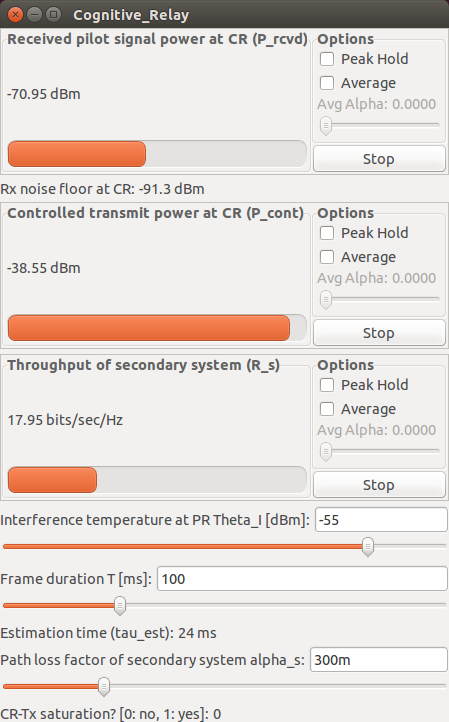
\includegraphics[width=0.5\textwidth]{figures/crinterface}
                };

                \begin{scope}[x={(image.south east)},y={(image.north west)}]
                \node[draw=none, fill=gray!08,font=\scriptsize] at (0.49,0.977) {Secondary Transmitter (CSC-BS)};
                \node[draw=none, fill=gray!08,font=\scriptsize, text width = 110, align = center] at (0.375,0.93) {Received power at the ST, $\eprcvdstpr$};
                \node[draw=none, fill=gray!08,font=\scriptsize, text width = 41, align = center] at (0.154,0.745) {Noise Floor};
                \node[draw=none, fill=gray!08,font=\scriptsize, text width = 102, align = center] at (0.349,0.69) {Control power at the ST, $\epreg$};
                \node[draw=none, fill=gray!08,font=\scriptsize, text width = 103, align =  center] at (0.352,0.50) {Secondary throughput at the SR, $\ers$};
                \node[draw=none, fill=gray!08,font=\scriptsize] at (0.356,0.28) {Interference temperature, $\ite$ = [dBm]};
                \node[draw=none, fill=gray!08,font=\scriptsize, text width = 48, align = center] at (0.176,0.20) {$T$ = [ms]};
                \node[draw=none, fill=gray!08,font=\scriptsize, text width = 54, align = center] at (0.196,0.125) {$\ttesto$ = [ms]};
                \node[draw=none, fill=gray!08,font=\scriptsize, text width = 102, align = center] at (0.349,0.08) {Access channel gain, $\hs$ = [mV]};

                %\draw[help lines,xstep=.1,ystep=.1] (0,0) grid (1,1);
                %\foreach \x in {0,1,...,9} { \node [anchor=north] at (\x/10,0) {0.\x}; }
                %\foreach \y in {0,1,...,9} { \node [anchor=east] at (0,\y/10) {0.\y}; }
                \end{scope}
        \end{tikzpicture}
	}	
	\caption{A snapshot of the performance parameters at the ST displayed by means of the graphical user interface.}
	\label{fig_HVD:interface_ST}
	%\vspace{-10 pt}
\end{figure}

\begin{figure}
	\centering
     	   \resizebox{0.65\textwidth}{!}{%
	   \begin{tikzpicture}[scale=1]
                \node[anchor=south west,inner sep=0] (image) at (0,0)
                {
			
\includegraphics[width=0.5\textwidth]{figures/printerface}
                };

                \begin{scope}[x={(image.south east)},y={(image.north west)}]
                \node[draw=none, fill=gray!35,font=\scriptsize] at (0.49,0.9712) {Primary Receiver};
                \node[draw=none, fill=gray!35,font=\scriptsize] at (0.352,0.92) {Interference Power at the PR, $\eprcvdpr$};
                \node[draw=none, fill=gray!35,font=\scriptsize] at (0.355,0.695) {Confidence probability constraint, $\pcod$};
                \node[draw=none, fill=gray!35,font=\scriptsize] at (0.25,0.45) {$\p(\eprcvdpr \ge \ite (1 + \acc))$};
                \node[draw=none, fill=gray!35,font=\scriptsize] at (0.25,0.21) {$\p(\eprcvdpr \le \ite (1 - \acc))$};
		
		%\draw[help lines,xstep=.1,ystep=.1] (0,0) grid (1,1);
                %\foreach \x in {0,1,...,9} { \node [anchor=north] at (\x/10,0) {0.\x}; }
                %\foreach \y in {0,1,...,9} { \node [anchor=east] at (0,\y/10) {0.\y}; }
                \end{scope}
        \end{tikzpicture}
	}
	\caption{A snapshot of the performance parameters at the PR displayed by means of the graphical user interface.}
	\label{fig_HVD:interface_PR}
	%\vspace{-10 pt}
\end{figure}

%\begin{figure}
%	\vspace{-15 pt}
%	\centering
%	\subfloat[User interface to the ST]
%	{
%		\begin{tikzpicture}[scale=1]
%                \node[anchor=south west,inner sep=0] (image) at (0,0)
%                {
%			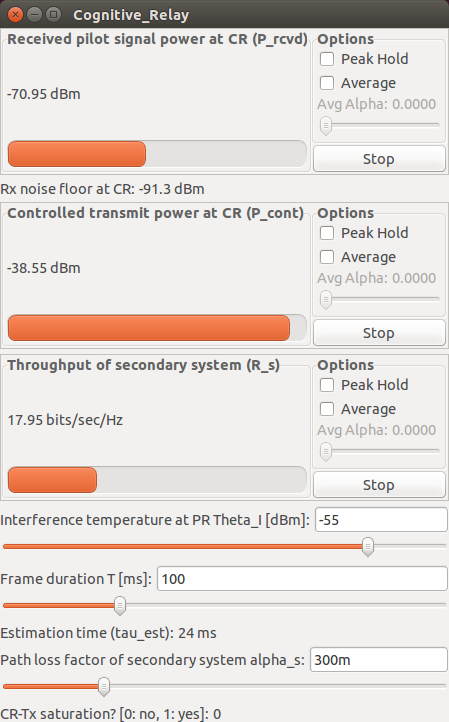
\includegraphics[width=0.5\textwidth]{figures/crinterface}
%                };
%
%                \begin{scope}[x={(image.south east)},y={(image.north west)}]
%                \node[draw=none, fill=gray!10,font=\scriptsize] at (0.49,0.977) {Secondary Transmitter (CSC-BS)};
%                \node[draw=none, fill=gray!10,font=\scriptsize, text width = 110pt, align = center] at (0.375,0.93) {Received power at the ST, $\eprcvdstpr$};
%                \node[draw=none, fill=gray!10,font=\scriptsize, text width = 41pt, align = center] at (0.154,0.745) {Noise Floor};
%                \node[draw=none, fill=gray!10,font=\scriptsize, text width = 102pt, align = center] at (0.349,0.69) {Control power at the ST, $\epreg$};
%                \node[draw=none, fill=gray!10,font=\scriptsize, text width = 103pt, align =  center] at (0.352,0.50) {Secondary throughput at the SR, $\ers$};
%                \node[draw=none, fill=gray!10,font=\scriptsize] at (0.356,0.28) {Interference temperature, $\ite$ = [dBm]};
%                \node[draw=none, fill=gray!10,font=\scriptsize, text width = 48pt, align = center] at (0.176,0.20) {$T$ = [ms]};
%                \node[draw=none, fill=gray!10,font=\scriptsize, text width = 54pt, align = center] at (0.196,0.125) {$\ttesto$ = [ms]};
%                \node[draw=none, fill=gray!10,font=\scriptsize, text width = 102pt, align = center] at (0.349,0.08) {Access channel gain, $\hs$ = [mV]};
%
%                %\draw[help lines,xstep=.1,ystep=.1] (0,0) grid (1,1);
%                %\foreach \x in {0,1,...,9} { \node [anchor=north] at (\x/10,0) {0.\x}; }
%                %\foreach \y in {0,1,...,9} { \node [anchor=east] at (0,\y/10) {0.\y}; }
%                \end{scope}
%        \end{tikzpicture}	
%	}\\[4pt]
%	\subfloat[User interface to the PR]{
%	   \begin{tikzpicture}[scale=1]
%                \node[anchor=south west,inner sep=0] (image) at (0,0)
%                {
%			
\includegraphics[width=0.5\textwidth]{figures/printerface}
%                };
%
%                \begin{scope}[x={(image.south east)},y={(image.north west)}]
%                \node[draw=none, fill=gray!40,font=\scriptsize] at (0.49,0.9712) {Primary Receiver};
%                \node[draw=none, fill=gray!40,font=\scriptsize] at (0.352,0.92) {Interference Power at the PR, $\eprcvdpr$};
%                \node[draw=none, fill=gray!40,font=\scriptsize] at (0.355,0.695) {Confidence probability constraint, $\pcod$};
%                \node[draw=none, fill=gray!40,font=\scriptsize] at (0.25,0.45) {$\p(\eprcvdpr \ge \ite (1 + \acc))$};
%                \node[draw=none, fill=gray!40,font=\scriptsize] at (0.25,0.21) {$\p(\eprcvdpr \le \ite (1 - \acc))$};
%		
%		%\draw[help lines,xstep=.1,ystep=.1] (0,0) grid (1,1);
%                %\foreach \x in {0,1,...,9} { \node [anchor=north] at (\x/10,0) {0.\x}; }
%                %\foreach \y in {0,1,...,9} { \node [anchor=east] at (0,\y/10) {0.\y}; }
%                \end{scope}
%        \end{tikzpicture}
%
%	}
%	\vspace{-12 pt}
%	\caption{A snapshot of the performance parameters displayed in the graphical user interface.}
%	\label{interface}
%	%\vspace{-10 pt}
%\end{figure}

Conversely, for the given accuracy $\acc = 0.05$, it is observed that the demonstrator fails to achieve the target value of the confidence probability constraint $\pcod = 0.95$. Certainly, this issue is largely caused due to the simplifications undertaken in Section \ref{ssec:simp2}. 
Also, in contrast to the hardware validation, for the demonstrator, the pilot signal is produced by a USRP, thus offering a poor signal quality than produced by the signal generator, deployed for the hardware validation. 
%Another possible reason for this kind of behaviour can be speculated as follows: Since a pilot signal produced by a signal generator has been used for the hardware validation, which offers a higher signal quality than the one produced by a USRP in the demonstrator. 
%Moreover, because of the separate links for sensing and transmission and the frequency separation of \SI{1}{MHz}, the channel reciprocity of the demonstrator may be compromised compared with the theoretical model. 

In order to tackle this violation of the confidence probability constraint, the proposed confidence probability constraint is sustained by increasing the tolerance limit to $\acc = 0.20$. 
As a result, the confidence probability reaches the target value $\pco = 0.95$, thereby satisfying the confidence probability constraint, refer to \figurename~\ref{fig_HVD:interface_PR}. 
To demonstrate a preliminary working of a CR system, these simplifications are affordable at this stage, however, it is important to relax these simplifications in the future work. 
Despite this deviation from the theoretical behaviour, it can be concluded that the USRPs, considered for the deployment, represent a viable choice for demonstrating the analysis, proposed in the thesis. 
Finally, to wrap up the discussions, the key observations while deploying the demonstrator for the US are summarized as follows: \begin{itemize} \item The deployed demonstrator reveals the necessity of the channel knowledge for the principle operation of a CR system in a practical situation. \item With the incorporation of channel estimation, the deployed hardware demonstrates the principle operation of an US that employs a power control mechanism at the ST, which is facilitated by performing received power-based channel estimation at the ST. \item Subsequently, the demonstrator clearly presents the effect of imperfect channel knowledge, in particular, the uncertain interference at the PR. In addition, it justifies the applicability of the confidence probability constraint at the ST, imposed for regulating the uncertain interference. 
\item Finally, the demonstrator illustrates the capability of adapting to the changes in the environment, particularly, in terms of the channel between the ST and the PR.  \end{itemize}
\index{Demonstrator|)}

\section{Summary}
\label{con}

In this chapter, the performance of an underlay system in consideration to a hardware implementation has been analyzed. To this end, an analytical framework has been validated by means of hardware measurements. 
%In this regard, the validation of a stochastic model that incorporates the pdfs of the system parameters has been considered. In addition, the performance analysis in terms of estimation-throughput tradeoff has been validated. 
In reference to the deployment process, it has been concluded that the knowledge of the interacting channels plays a crucial role in the hardware realization of the CR systems, the main aspect outlined in the thesis. Following the validation process, it has been justified that the proposed analysis that incorporates the received power-based estimation for the links between the primary and the secondary systems, proposed in the thesis, facilitates the hardware feasibility of a CR system by supporting low complexity and the versatility towards unknown primary user signals. Based on the experimental validation, a hardware demonstrator that depicts the principle working of the underlay system has been examined. 

More importantly, in this chapter, the major challenges such as \begin{itemize} \item a certain pre-processing to exclude spurious effects, affecting the hardware validation of the derived expressions, \item a careful selection of the estimation time for a given operation regime defined in terms of signal to noise ratio received at the SR, \item a proper implementation of the power control and \item a simplified approach to workaround channel reciprocity, \end{itemize} considered while deploying the demonstrator, have been discussed adequately. Consequently, the corresponding solutions and simplifications to overcome these challenges have been proposed.  


%In the future, we intend to reconsider certain simplifications made while deploying the demonstrator, for instance, we propose to deploy a USRP for the SR and try to synchronize the frame structure at the ST and the PR in order to respect channel reciprocity.












%Implementation using software defined radio.
%\section{Interweave system}
%
%\subsection{System model}
%
%\subsection{Measurement setup}
%\begin{figure}[!t]
%        \centering
%        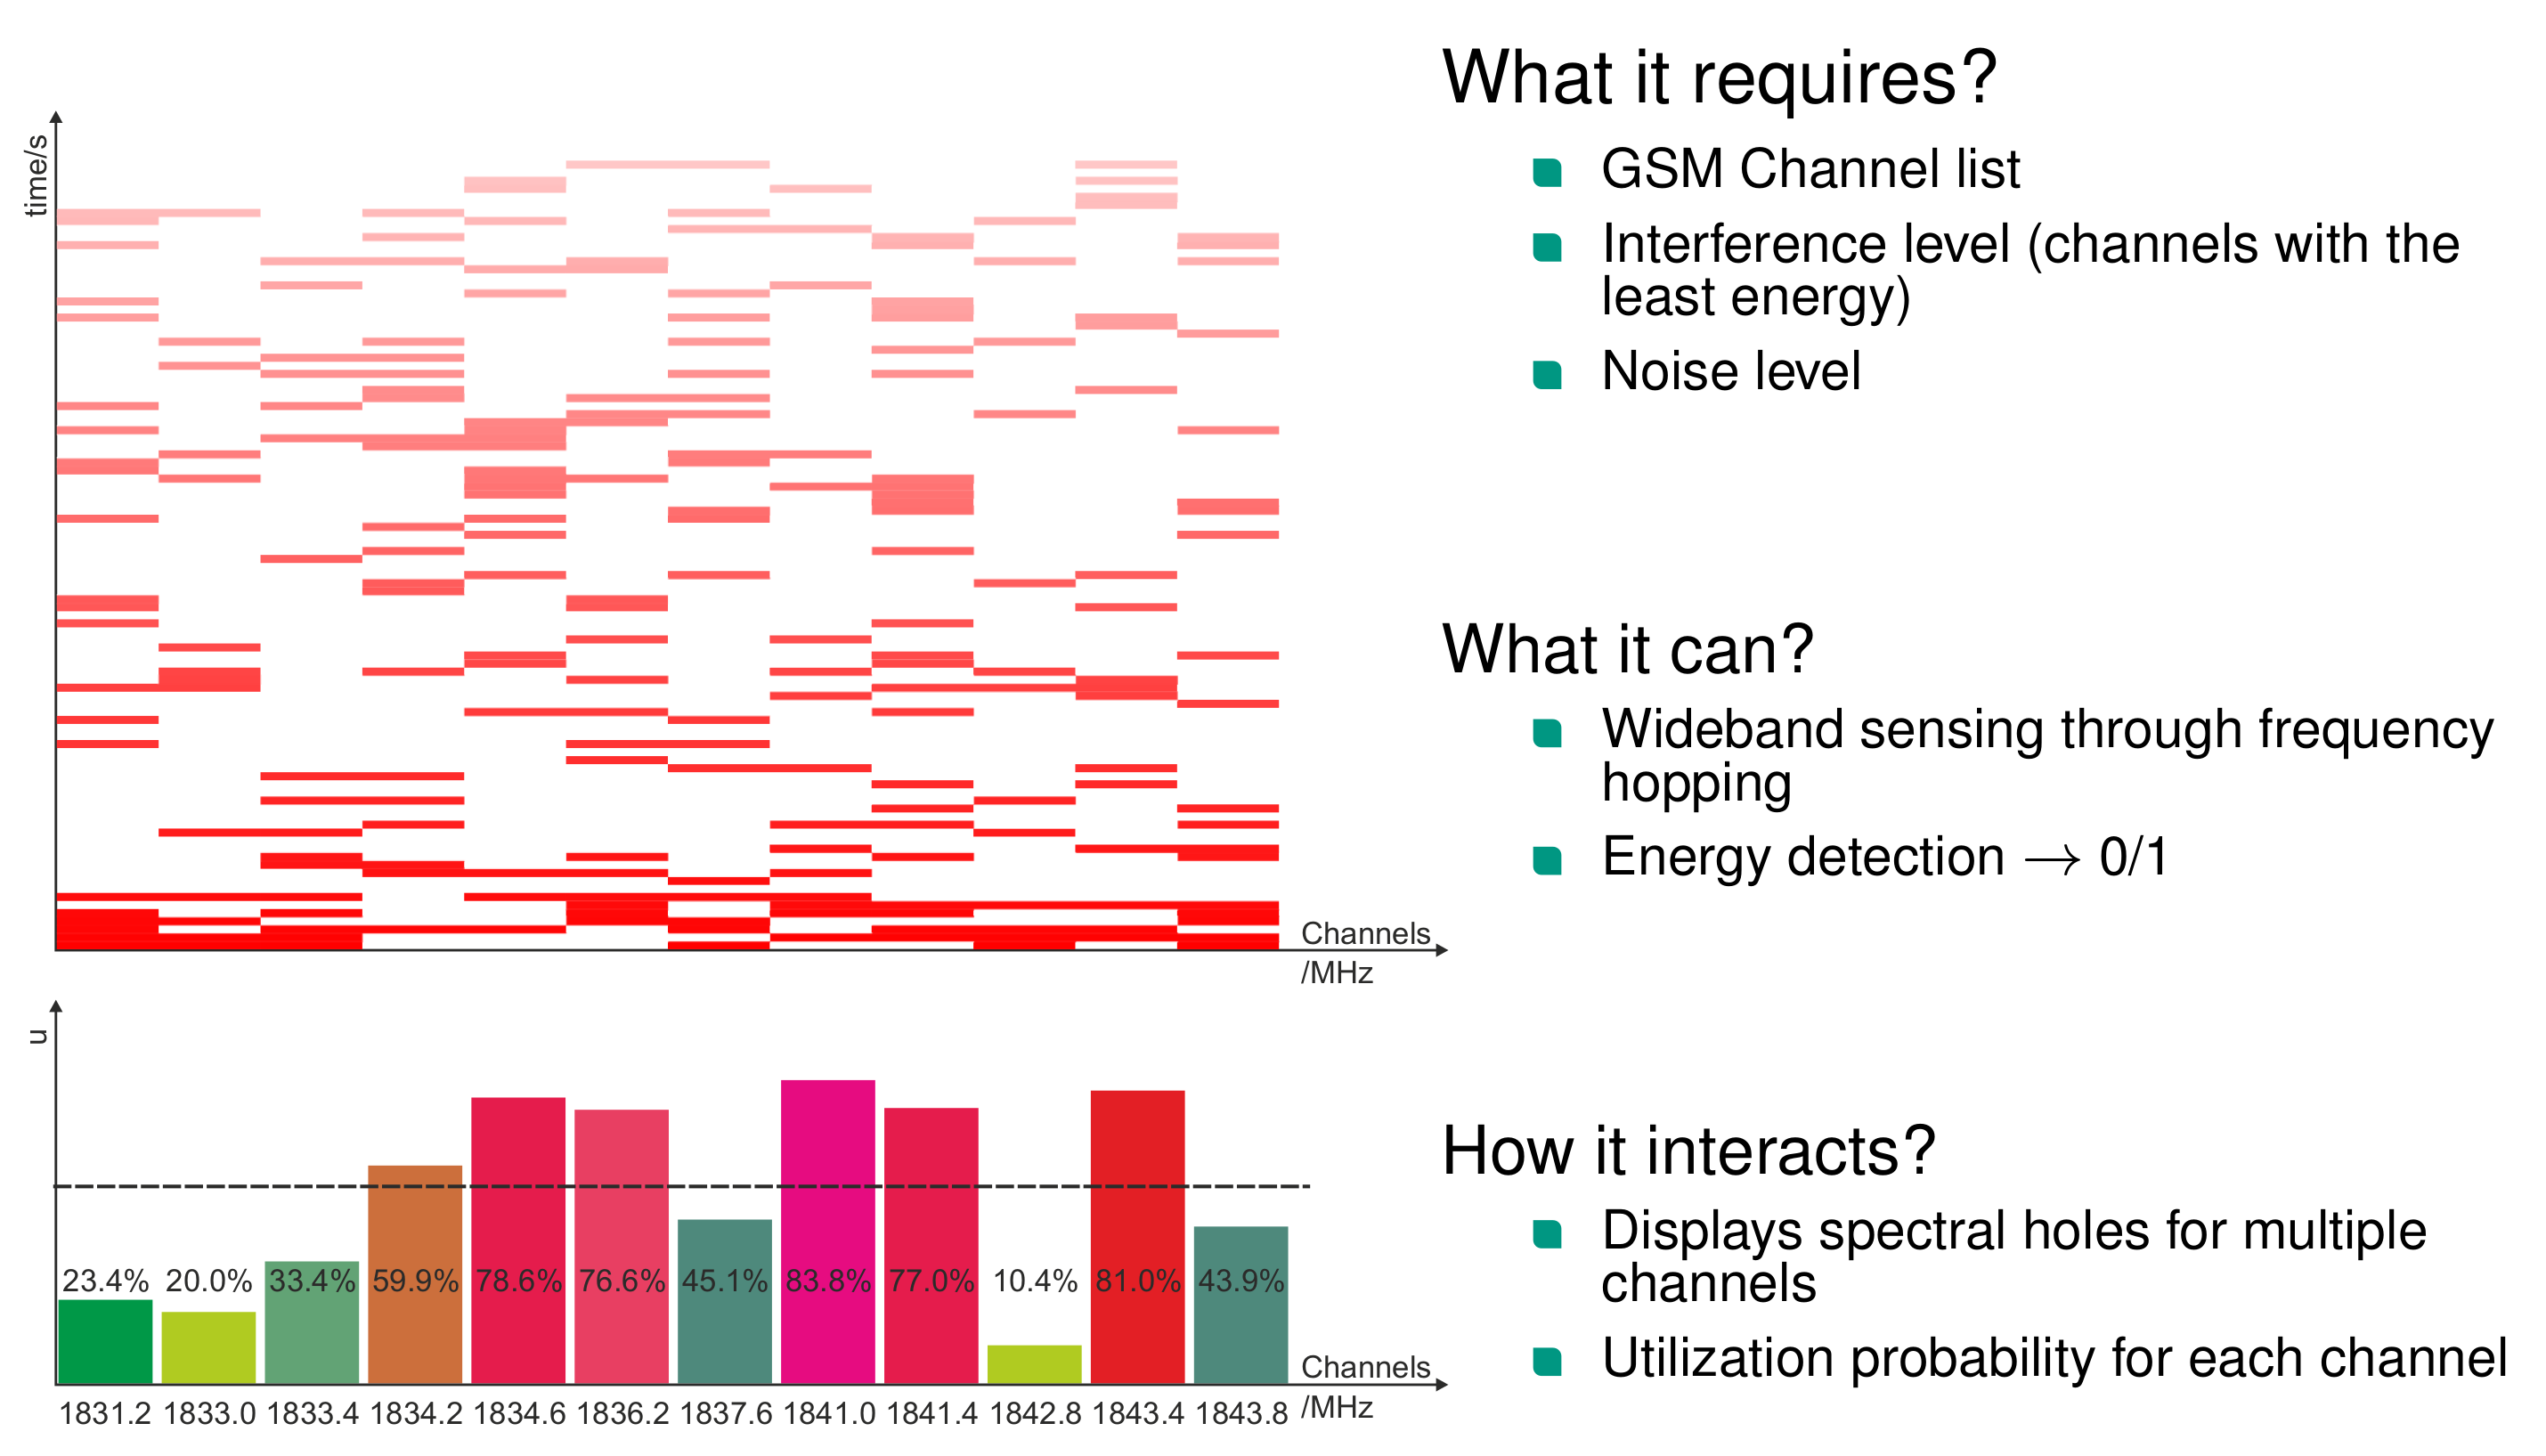
\includegraphics[trim=0.0cm 0.0cm 5.28cm 0.0cm,clip=true,width=\columnwidth]{../kapitel05/figures/Interweave_GUI.png}
%        \caption{Utilization probability for ranking the GSM subchannels.}
%        \label{fig_HVD:uti}
%\end{figure}
%Hardware demonstration \cite{Kaushik_ISWCS} of \ac{CR} that
%\begin{itemize}
%\item detects spectrum holes or temporal opportunities in \ac{PU} system 
%\item illustrates cognitive sensing ,i.e, it estimates the spectral occupancy for the multi-band \ac{PU} system
%\end{itemize}
%
%\subsection{Analysis}
%
%\section{Underlay system}
%
%\subsection{System model}
%CR models the channel coefficients $h_\text{p}$, $h_\text{s}$, using Rayleigh or Nakagami-$m$ distribution for the indoor-indoor and indoor-outdoor links. In literature, Rayleigh distribution is mostly preferred due to its analytical tractability. In contrast to that, Nakagami-$m$ accounts for the severity in fading through $m$ parameter, thus, it is more applicable in indoor scenarios. For a fixed transmit power at CR, the received signal to noise power $\gamma$\footnote{Consider a transmission from a certain CR, then $\gamma$ is equivalent to signal to noise ratio (SNR) at ID and interference to noise ratio at PR. Therefore, the term SNR is not used to avoid confusion thereof. Moreover, the interference from unintended primary transmitters and other CRs at PR or ID is treated as white noise.} at PR or ID, corresponding to Rayleigh case, follows exponential distribution \cite{simon2005}
%\begin{equation}
%\label{eq_HVD:expo}
%F_{\gamma}(\gamma) = 1 - e^{- \frac{\gamma}{\bar{\gamma}} }
%\end{equation}
%and for Nakagami-$m$, it follows Gamma distribution \cite{simon2005}
%\begin{equation}
%\label{eq_HVD:gamma}
%F_{\gamma}(\gamma) = 1 - \frac{ \Gamma{ \left( m, m \frac{\gamma}{\bar{\gamma}} \right) }}{\Gamma(m)},
%\end{equation}
%where $\bar{\gamma} = \mathbb{E}[\gamma]$ and $m$ denotes the shape parameter. $\Gamma(\cdot)$ and $\Gamma(\cdot,\cdot)$ are the complete and incomplete Gamma functions. 
%
%
%\begin{figure}[!t]
%        \centering
%        \includegraphics[width = \columnwidth]{../kapitel05/figures/wo_channels_CR_Scenario_farbig_general}
%        \caption{A scenario demonstrating the interaction between the PU and the CR. The CR senses PUs channels in the outdoor to provide a dynamic access to the devices operating indoor.}
%        \label{fig_HVD:scenario}
%\end{figure}
%
%\begin{figure}[!t]
%        \centering
%        \includegraphics[width = 0.8\columnwidth]{../kapitel05/figures/setup}
%        \caption{Hardware setup.}
%        \label{fig_HVD:hw_setup}
%\end{figure}
%
%
%\ac{CR} operating as underlay system \cite{Kaushik_CROWNCOM}
%\begin{itemize}
%\item deploys propagation models to capture movements of \ac{PR} and \ac{ID}
%\item implements sharing constraints to access the \ac{PU} channel 
%\end{itemize}
%
%\subsection{Measurement setup}
%\begin{figure}[!t]
%        \centering
%        \includegraphics[width = \columnwidth]{../kapitel05/figures/floor_B}
%        \caption{The deployment scenario for the CR including ID and PR at different spatial positions. The circle around the PR and ID positions represents $\mathbb{R}$, which illustrates their small movements.}
%        \label{fig_HVD:deploymentScenario}
%\end{figure}
%
%\begin{figure}[!t]
%        \centering
%        \includegraphics[width = 0.8\columnwidth]{../kapitel05/figures/setup}
%        \caption{Hardware setup.}
%        \label{fig_HVD:hw_setup}
%\end{figure}
%
%\subsection{Analysis}
%
%\subsubsection{\ac{IC} at PR}
%
%\begin{table}
%\renewcommand{\arraystretch}{1.3}
%\caption{Parameters and MSE of the $F_{I}$ modeled using Rayleigh and Nakagami-$m$ distribution for different PR positions}
%\label{tb_HVD:MSE_II}
%\centering
%\begin{tabular}{c||c|c}
%\hline
%\bfseries Outdoor & \bfseries Rayleigh (\ref{eq_HVD:expo}) & \bfseries Nakagami-$m$ (\ref{eq_HVD:gamma}) \\
%\bfseries Position & [MSE, $\widehat{\bar{\gamma}}]$ & [MSE, $(\widehat{m}, \widehat{\bar{\gamma}}$)] \\
%\hline\hline
%PR1 & $[3.84 \cdot 10^{-4}, 2.66 \cdot 10^{2} ]$  & $[1.74 \cdot 10^{-4} , (1.13, 2.66 \cdot 10^{2})] $ \\ \hline
%PR2 & $[2.75 \cdot 10^{-4}, 4.89 \cdot 10^{2}]$  & $[2.40 \cdot 10^{-4} , (0.98, 4.89 \cdot 10^{2})] $ \\ \hline
%PR3 & $[2.75 \cdot 10^{-4}, 57.34]$  & $[2.31 \cdot 10^{-4} , (1.11, 57.34)] $ \\ \hline
%PR4 & $[9.36 \cdot 10^{-4}, 94.20]$  & $[2.18 \cdot 10^{-4} , (1.25, 94.20)] $ \\ \hline
%\end{tabular}
%\end{table}
%
%
%\subsubsection{\ac{CC} at ID}
%
%\begin{figure}%
%\centering
%\begin{tikzpicture}[scale = 1.2]
%\node[anchor=south west,inner sep=0] (image) at (0,0)
%{\includegraphics[trim=1.5cm 0.4cm 1.45cm 1.2cm,clip=true,width=\columnwidth]{../kapitel05/figures/Interference_CDF_ana_vs_sim_indoor_outdoor}};
%\begin{scope}[x={(image.south east)},y={(image.north west)}]
%\draw  (0.832,0.99) node[above=-0.1pt, font=\small] {$I_{\text{th}}$};
%\draw  (.97,0.898) node[right=-2.2pt, font=\small] {$\epsilon_{\text{I,out}}$};
%\draw[black,thick,<->] (0.97,0.898) --  node[right=-2.2pt, font=\small] {$\epsilon_{\text{I,out}}$} (0.97,0.985);
%\draw [thick] (0.831,0.985) -- (0.831,0.096);
%\draw [thick] (0.08,0.898) -- (0.956,0.898);
%
%%Select channels for based on Interference Constraint   
%\draw (0.675,0.85) ellipse(24pt and 5pt)  node[left=28pt, font=\small] {IC};
%\draw[help lines,xstep=.1,ystep=.1] (0,0) grid (1,1);
%\foreach \x in {0,1,...,9} { \node [anchor=north] at (\x/10,0) {0.\x}; }
%\foreach \y in {0,1,...,9} { \node [anchor=east] at (0,\y/10) {0.\y}; }
%\end{scope}
%\end{tikzpicture}
%\caption{Interference distribution function at different PR positions.}
%\label{subfig_HVD:indoor-outdoor}
%\end{figure}
%
%\begin{figure}
%\centering
%\begin{tikzpicture}[scale = 1.2]
%\node[anchor=south west,inner sep=0] (image) at (0,0)
%{\includegraphics[trim=1.5cm 0.4cm 1.45cm 1.2cm,clip=true,width=\columnwidth]{../kapitel05/figures/Capacity_CDF_ana_vs_sim_indoor_indoor}};
%\begin{scope}[x={(image.south east)},y={(image.north west)}]
%\draw  (0.255,0.99) node[above=-0.1pt, font=\small] {$C_{\text{th}}$};
%\draw  (.97,0.178) node[right=-2.2pt, font=\small] {$\epsilon_{\text{C,out}}$};
%\draw[black,thick,<->] (0.97,0.095) --  node[right=-2.2pt, font=\small] {$\epsilon_{\text{C,out}}$} (0.97,0.186);
%\draw [thick] (0.255,0.985) -- (0.255,0.096);
%\draw [thick] (0.08,0.186) -- (0.956,0.186);
%Select channels for based on Capacity Constraint       
%\draw (0.48,0.58) ellipse (38pt and 5pt)  node[right=48 pt, font=\small] {CC};
%\draw[help lines,xstep=.1,ystep=.1] (0,0) grid (1,1);
%\foreach \x in {0,1,...,9} { \node [anchor=north] at (\x/10,0) {0.\x}; }
%\foreach \y in {0,1,...,9} { \node [anchor=east] at (0,\y/10) {0.\y}; }
%\end{scope}
%\end{tikzpicture}
%\label{subfig_HVD:indoor-indoor}
%\end{figure}
%
%\begin{table}
%\renewcommand{\arraystretch}{1.3}
%\caption{Parameters and MSE of the $F_{C}$ modeled using Rayleigh and Nakagami-$m$ distribution for different ID positions}
%\label{tb_HVD:MSE_IO}
%\centering
%\begin{tabular}{c||c|c}
%\hline
%\bfseries Indoor & \bfseries Rayleigh (\ref{eq_HVD:expo}) & \bfseries Nakagami-$m$ (\ref{eq_HVD:gamma}) \\
%\bfseries Position & [MSE, $\widehat{\bar{\gamma}}]$ & [MSE, $(\widehat{m}, \widehat{\bar{\gamma}}$)] \\
%\hline\hline
%ID1 & $[1.11 \cdot 10^{-3}, 9.52 \cdot 10^{2}]$  & $[1.74 \cdot 10^{-4} , (1.23, 9.52 \cdot 10^{2})] $ \\ \hline
%ID2 & $[1.60 \cdot 10^{-3}, 3.65 \cdot 10^{4}]$  & $[3.39 \cdot 10^{-4} , (1.28, 3.65 \cdot 10^{4})] $ \\ \hline
%ID3 & $[5.79 \cdot 10^{-4}, 1.79 \cdot 10^{2}]$  & $[1.35 \cdot 10^{-4} , (1.17, 1.79 \cdot 10^{2})] $ \\ \hline
%ID4 & $[9.35 \cdot 10^{-4}, 4.13 \cdot 10^{2}]$  & $[3.05 \cdot 10^{-4} , (1.16, 4.13 \cdot 10^{2})] $ \\ \hline
%ID5 & $[7.54 \cdot 10^{-4}, 6.99 \cdot 10^{4}]$  & $[2.96 \cdot 10^{-4} , (1.23, 6.99 \cdot 10^{4})] $ \\ \hline
%\end{tabular}
%\end{table}
%
%
%\begin{table}[!h]
%\renewcommand{\arraystretch}{1.3}
%\caption{Cognitive relay implementing AND rule for different PR and ID positions}
%\label{tb_HVD:BDecisions}
%\centering
%\begin{tabular}{c||c|c|c|c}
%\hline
%\bfseries & PR1 & PR2 & PR3 & PR4 \\
%\hline\hline
%ID1 & 1 $\cdot$ 0 = 0 & 0 $\cdot$ 0 = 0 & 1 $\cdot$ 0 = 0 & 1 $\cdot$ 0 = 0 \\ \hline
%ID2 & 1 $\cdot$ 1 = 1 & 0 $\cdot$ 1 = 0 & 1 $\cdot$ 1 = 1 & 1 $\cdot$ 1 = 1 \\ \hline
%ID3 & 1 $\cdot$ 1 = 1 & 0 $\cdot$ 1 = 0 & 1 $\cdot$ 1 = 1 & 1 $\cdot$ 1 = 1 \\ \hline
%ID4 & 1 $\cdot$ 0 = 0 & 0 $\cdot$ 0 = 0 & 1 $\cdot$ 0 = 0 & 1 $\cdot$ 0 = 0 \\ \hline
%ID5 & 1 $\cdot$ 1 = 1 & 0 $\cdot$ 1 = 0 & 1 $\cdot$ 1 = 1 & 1 $\cdot$ 1 = 1 \\ \hline
%\end{tabular}
%\end{table}




